\documentclass[DIN, pagenumber=false, fontsize=11pt]{scrartcl}
\usepackage[utf8]{inputenc}
\usepackage{listings}
\usepackage{amssymb}
\usepackage{stmaryrd}
\usepackage{ulem}
\usepackage{enumerate}
\usepackage{amsmath}
%\usepackage{pgf-umlsd}
%\usepackage{tikz-er2}
\usepackage{enumitem}
\usepackage{graphicx}

\usepackage{etoolbox,fancyhdr}% http://ctan.org/pkg/{etoolbox,fancyhdr}

\fancyhf{}% Clear header/footer    
\fancyhead[R]{\thepage}% Page number in Right header
\fancyhead[L]{Bericht \thesection, QC-Toolkit}% \leftmark in Left header
\pagestyle{fancy}

\makeatletter
\patchcmd{\l@section}{#1}{#1}{}{}% Correct ToC
\renewcommand{\sectionmark}[1]{\markboth{Bericht \thesection, QC-Toolkit}{}}% Header mark
\renewcommand{\@seccntformat}[1]{\csname the#1\endcsname}% Correct in-text \section # format
\let\oldsection\section% Store \section in \oldsection
\makeatother
\renewcommand{\section}[1]{\oldsection[]{#1}}% Sections don't have a title in the ToC

\setcounter{section}{1} %Set up the actual exercise
\setcounter{subsection}{0} %Set up the actual exercise-1

\newcommand{\mytitle}[1]{{\noindent\Large\textbf{#1}}}
\newcommand{\mysection}[1]{\textbf{\section*{#1}}}

\title{Vorbesprechung QC-Toolkit}
\date{20.02.2015}
\author{Jerome Bergmann \\ Lukas Prediger}

\begin{document}

\noindent\textbf{QC-Toolkit} \hfill \textbf{RWTH Aachen}\\
Jerome Bergmann \hfill \textbf{Anfang:} 12:30, \textbf{Ende:} 15:30 \\
Lukas Prediger  \hfill \textbf{Nächster Termin:} 03.03.2015, 10:00\\
Außerdem Anwesend: Deni Raco, Evgeni Wachnowezki, Simon Humpohl\\

\mytitle{Bericht \thesection \hfill 20.02.2015}

\subsection{ Experiment: }
\begin{itemize}[noitemsep]
	\item Quantenzustand eines Qubits wird über einen Spannungsverlauf (Steuersignal) manipuliert
	\item Auswirkungen des Steuersignalverlaufs auf Quantenzustand soll untersucht werden
	\item Verschiedene Geräte für Ausgabe des Steuersignals (AWG) und Messung des Quantenzustands vorhanden
	\begin{itemize}[noitemsep]
		\item grundsätzlich voneinander unabhängig
		\item hardwareseitig zeitlich synchronisiert (durch sog. Marker)
	\end{itemize}
	\item Messzeitpunkte hängen vom Steuersignal ab (Steuersignal muss Messzeiträume berücksichtigen und zu diesen einen bestimmten Spannungswert halten/annehmen)
	\item Steuersignal wird logisch unterteilt in Pulse, kurze Spannungsverläufe die eine bestimmte Veränderung des Quantenzustands bewirken
	\item In einem Messlauf wird ein Spannungsverlauf mehrfach gemessen, um statistisch tragbare Daten zu erhalten
	\item Problem: Steuersignal und Messgeräte müssen unabhängig voneinander konfiguriert werden, aber so, dass an sinnvollen Stellen gemessen wird
\end{itemize}

\subsection{ Vorhandene Software: }
\begin{itemize}[noitemsep]
	\item gesplittet in zwei Module: specialmeasure und pulsecontrol
	\item specialmeasure: Erlaubt die Konfiguration der Messgeräte und die Durchführung von Messläufen (sog. Scanlines)
	\item pulsecontrol: Erlaubt die Konfiguration von Steuersignalen/Pulsen und den Upload auf AWG-Geräte
	\item Momentan stellen beide Module Funktionen bereit, die auf structs arbeiten.
	\item Globale Daten beider Frameworks stehen auch in structs bereits (smdata, plsdata, awgdata)
\end{itemize}

\subsubsection{ Pulse: }
\begin{itemize}[noitemsep]
 \item Werden für Hardware dargestellt als Waveform: Spannungssequenz über Zeit
 \item specialmesaure erlaubt verschiedene Definitionsmöglichkeiten (Waveform, pulsetab, weitere)
 \begin{itemize}[noitemsep]
 	\item pulsetab: Sequenz von Punkten (Zeit,Spannungsamplitude) aus denen dann die Waveform mittels linearer Interpolation generiert wird
 \end{itemize}
 \item Pulsgruppen sind Sequenzen von Pulsen oder Pulsgruppen und können parametrisierbar sein (z.B. Amplitude, Wartezeiten..)
 \item Pulse werden persistent in einer Datei abgelegt und haben eine eindeutige ID
 \item Pulse können verschiedene Ausgabespannungen für verschiedene Kanäle definieren
\end{itemize}
\paragraph{ Struct Pulsgruppe (pg): }
\begin{itemize}[noitemsep]
 \item Name: \texttt{pg.name}
 \item Puls: \texttt{pg.pulses} (Identifiziert über ID)
 \item \# Wiederholungen: \texttt{pg.nrep} 
 \item Kanäle: \texttt{pg.chan} : Mapping von den in Pulsen definierten Kanälen. Z.B.: Muster (initially ex. [1,2]) invertieren [2,1]
\end{itemize}
Puls und \# Wiederholungen können sowohl einzelne Werte, als auch Arrays von werten sein.

\subsubsection{ Schlüsselfunktionen: }
\begin{itemize}[noitemsep]
 \item \texttt{awgadd(struct pulsgruppe)}: Lädt Pulsgruppe als Waveform auf den AWG
 \item \texttt{smrun()}: Startet eine Scanline
\end{itemize}

\subsubsection{ Spezifikationsdetails:}
\begin{itemize}[noitemsep]
 \item \texttt{uint16} wird als Ein- und Ausgabetyp für Hardware verwendet. Intern wird bei PXDAC/Tectronic \texttt{uint10}/\texttt{uint14} verwendet.
 \item Matlab verwendet standardmäßig immer \texttt{double}
\end{itemize}

\subsubsection{ Hardwaretreiber: }
\begin{itemize}[noitemsep]
  \item Objektorientierte Umsetzung der Hardwaretreiber momentan in Arbeit
  \item AWG-Gerätetreiber werden durch abstrakte Klasse AWG abstrahiert
  \item Klasse VAWG: Abstraktionsebene: Fasst mehrere AWG-Instanzen als einen virtuellen AWG zusammen (zwecks Rückwärtskompatibilität mit aktuellem Code)
\end{itemize}

\subsection{ Wortschatz}
\begin{itemize}[noitemsep]
 \item Waveform ist ein Puls: (Wird generiert (Endvektor))
 \item Pulstab: Punktweise angabe (Dazwischen wird interpoliert)
 \item Scanline: Ein Messvorgang (1x SMRun)
 \item VAWG: virtueller AWG, bestehend aus mehereren AWG, die ein großes Setup darstellen (abstraktionsebene) (AWG)
 \item PXDAC (PCI-Bus): Gerät lädt modulationen in den RAM und kann nur von REG A bis REG B n mal abspielen
 \item Measure enspricht einem Puls der ausgemessen wird(hier werden die Werte dann zB gemittelt) 
\end{itemize}

\subsection{ Bilder}
\begin{figure}[h]
\begin{center}
 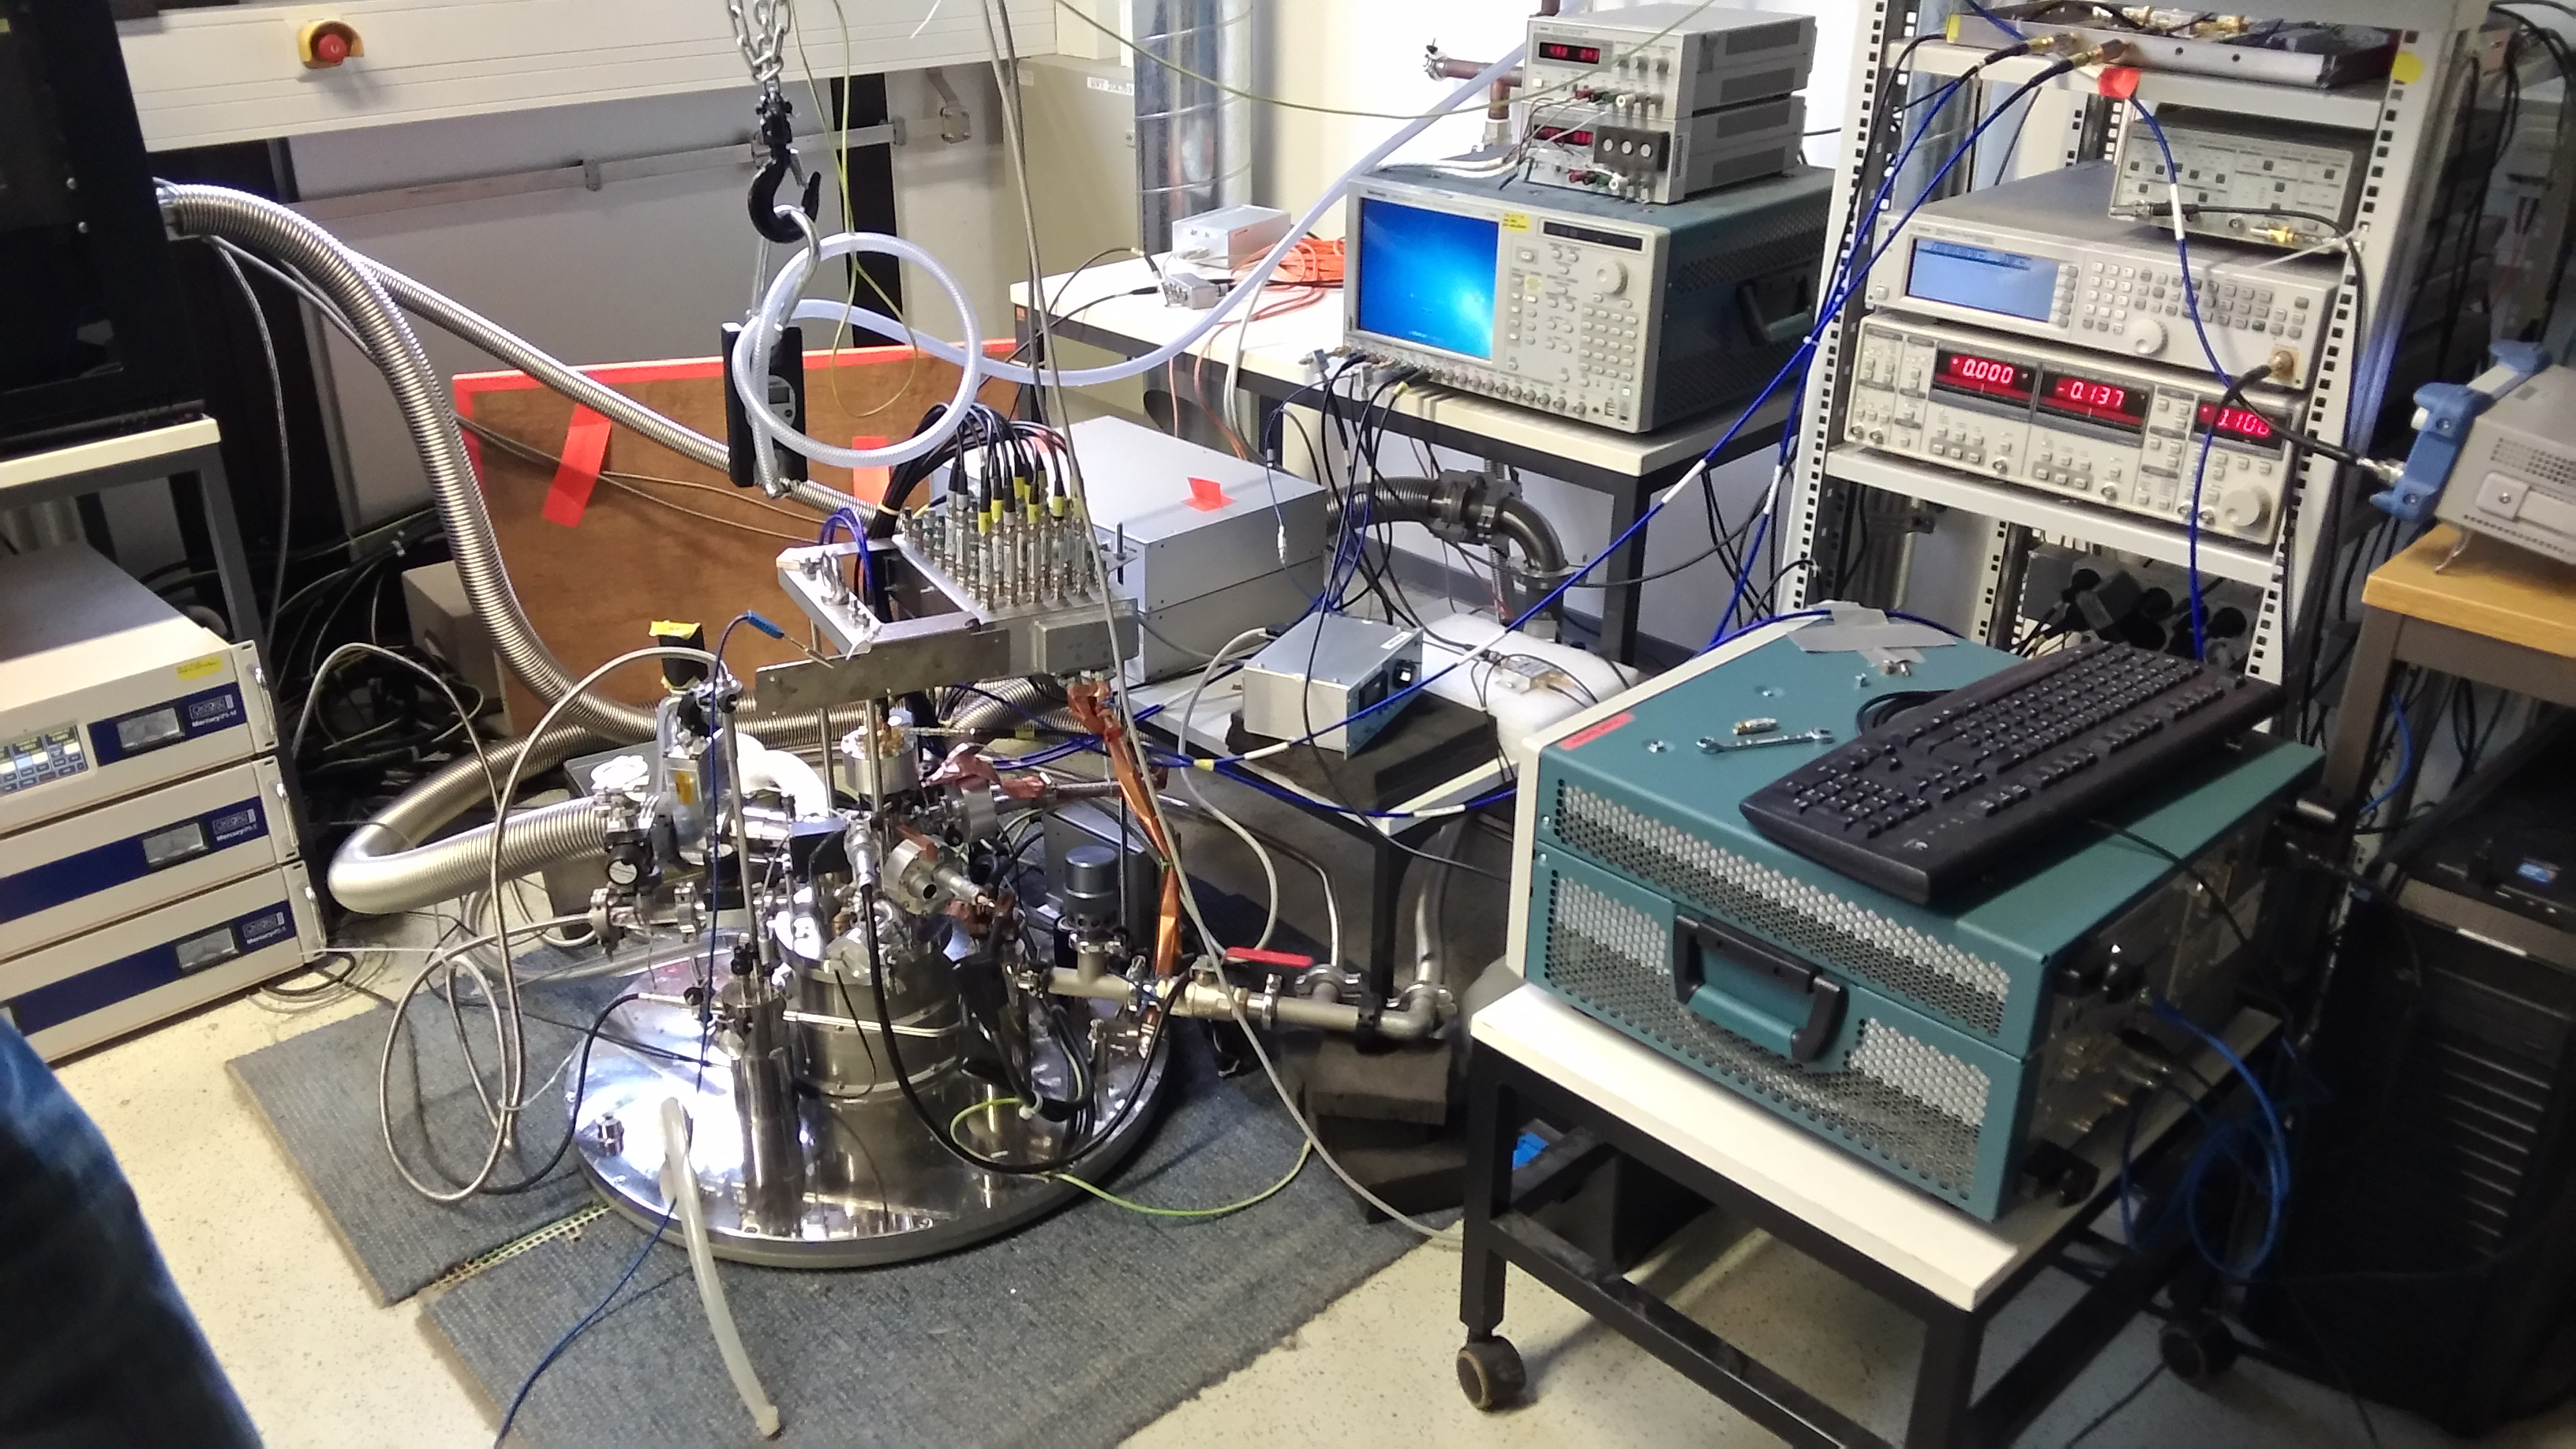
\includegraphics[width=.75\textwidth]{pictures/P_20150225_142624.jpg} \qquad
 \caption{Der Versuchsaufbau}
\end{center}
\end{figure}

\begin{figure}[h]
\begin{center}
 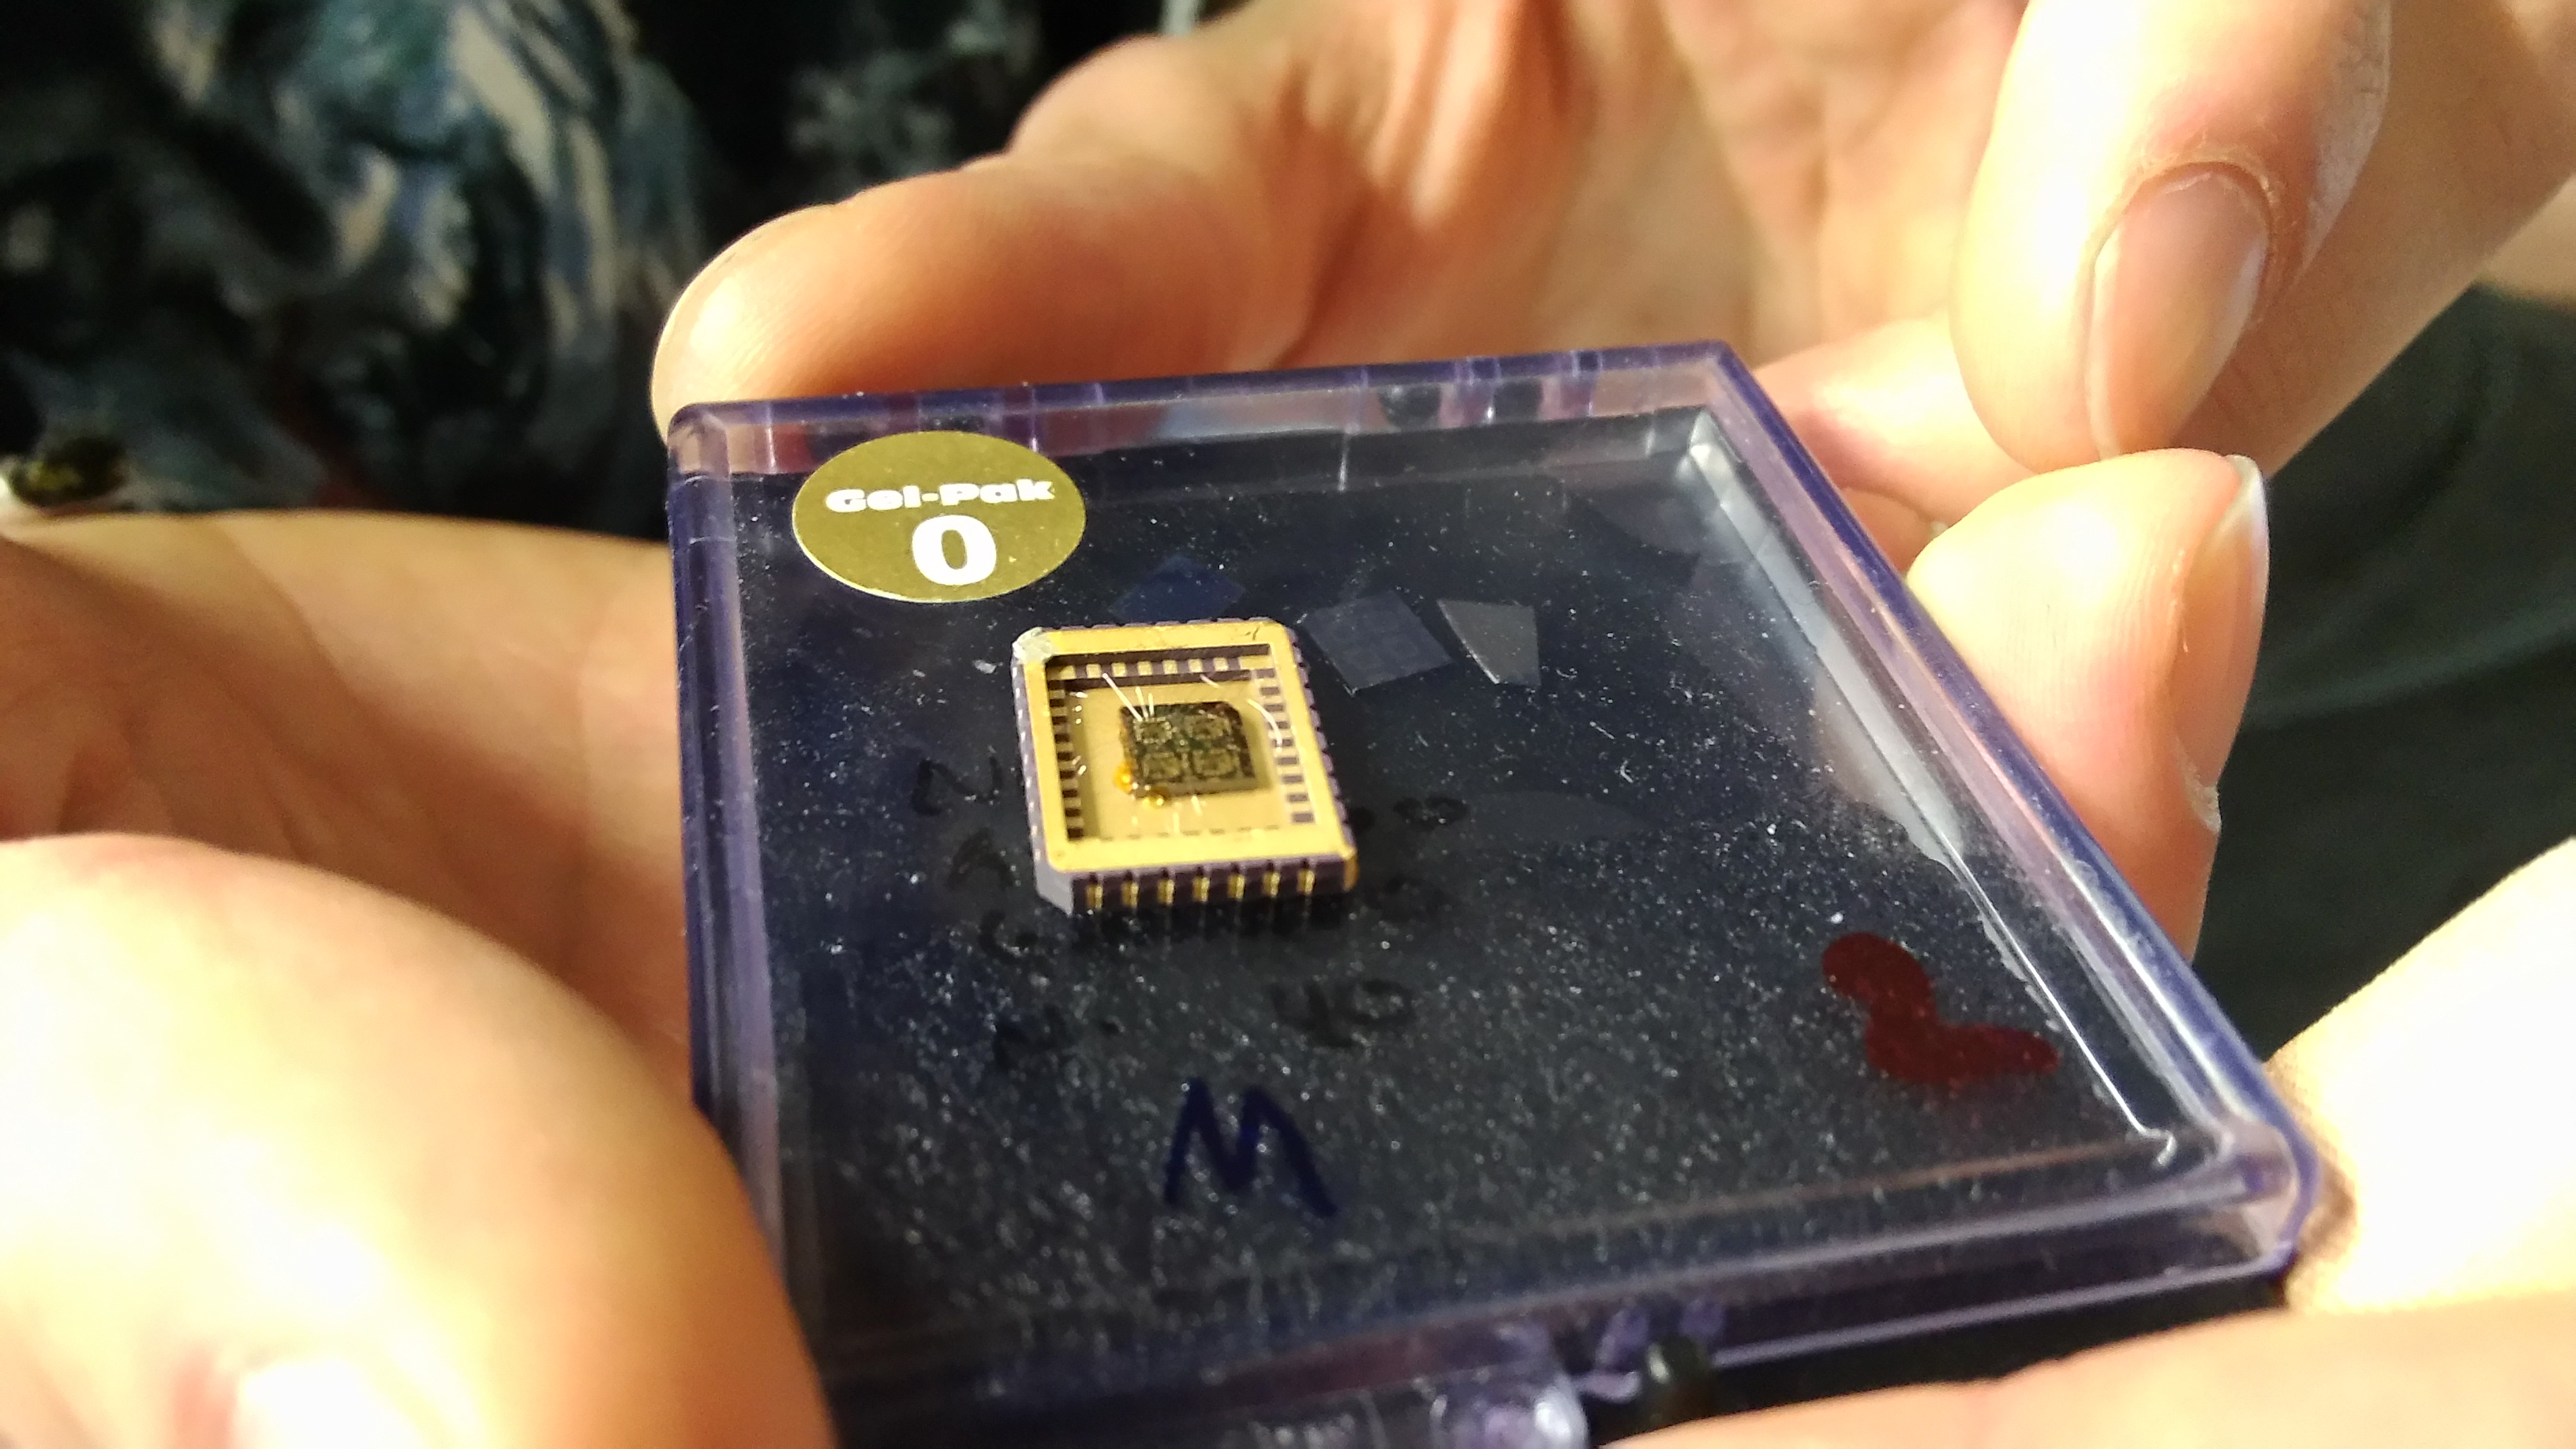
\includegraphics[width=.75\textwidth]{pictures/P_20150225_142709.jpg} \qquad
 \caption{Der Chip auf dem 4 Qubits realisiert weden}
\end{center}
\end{figure}

\begin{figure}[h]
\begin{center}
 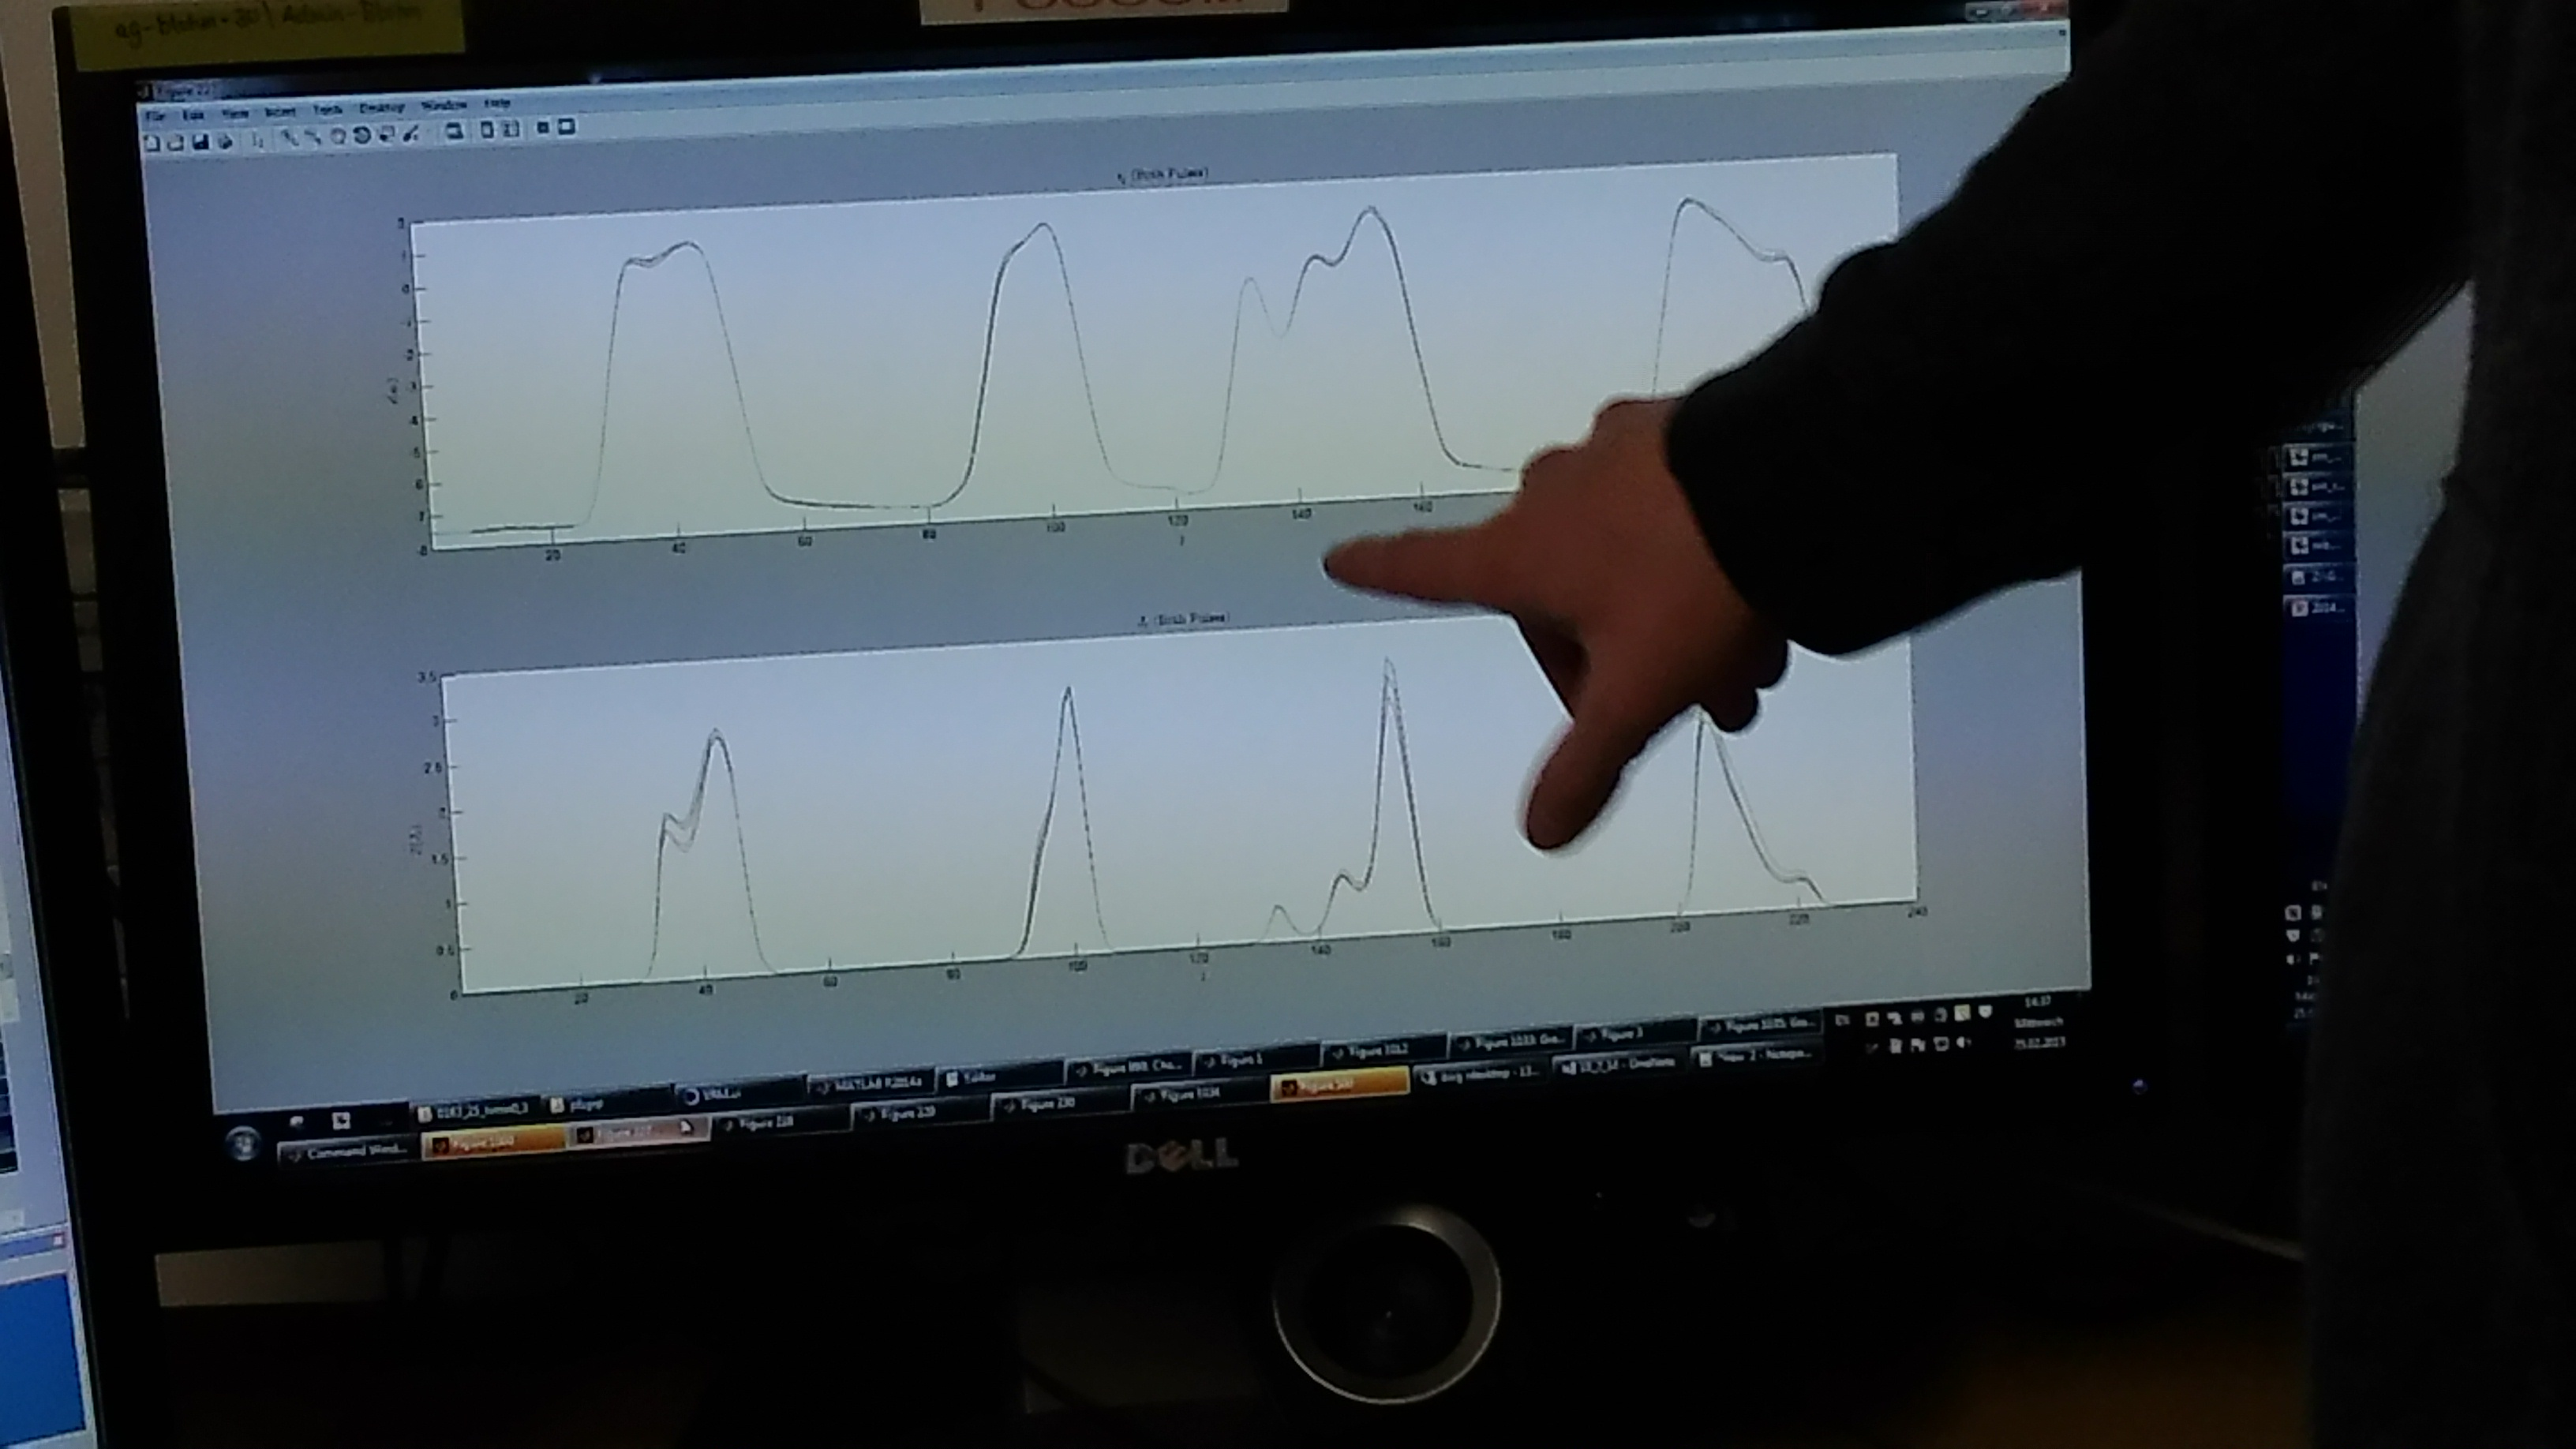
\includegraphics[width=\textwidth]{pictures/P_20150225_143702.jpg} \qquad
 \caption{Die hochgeladene Waveform kann als Spannungsverlauf auf dem Computer betrachtet werden}
\end{center}
\end{figure}

% \begin{figure}[h]
% \begin{center}
%  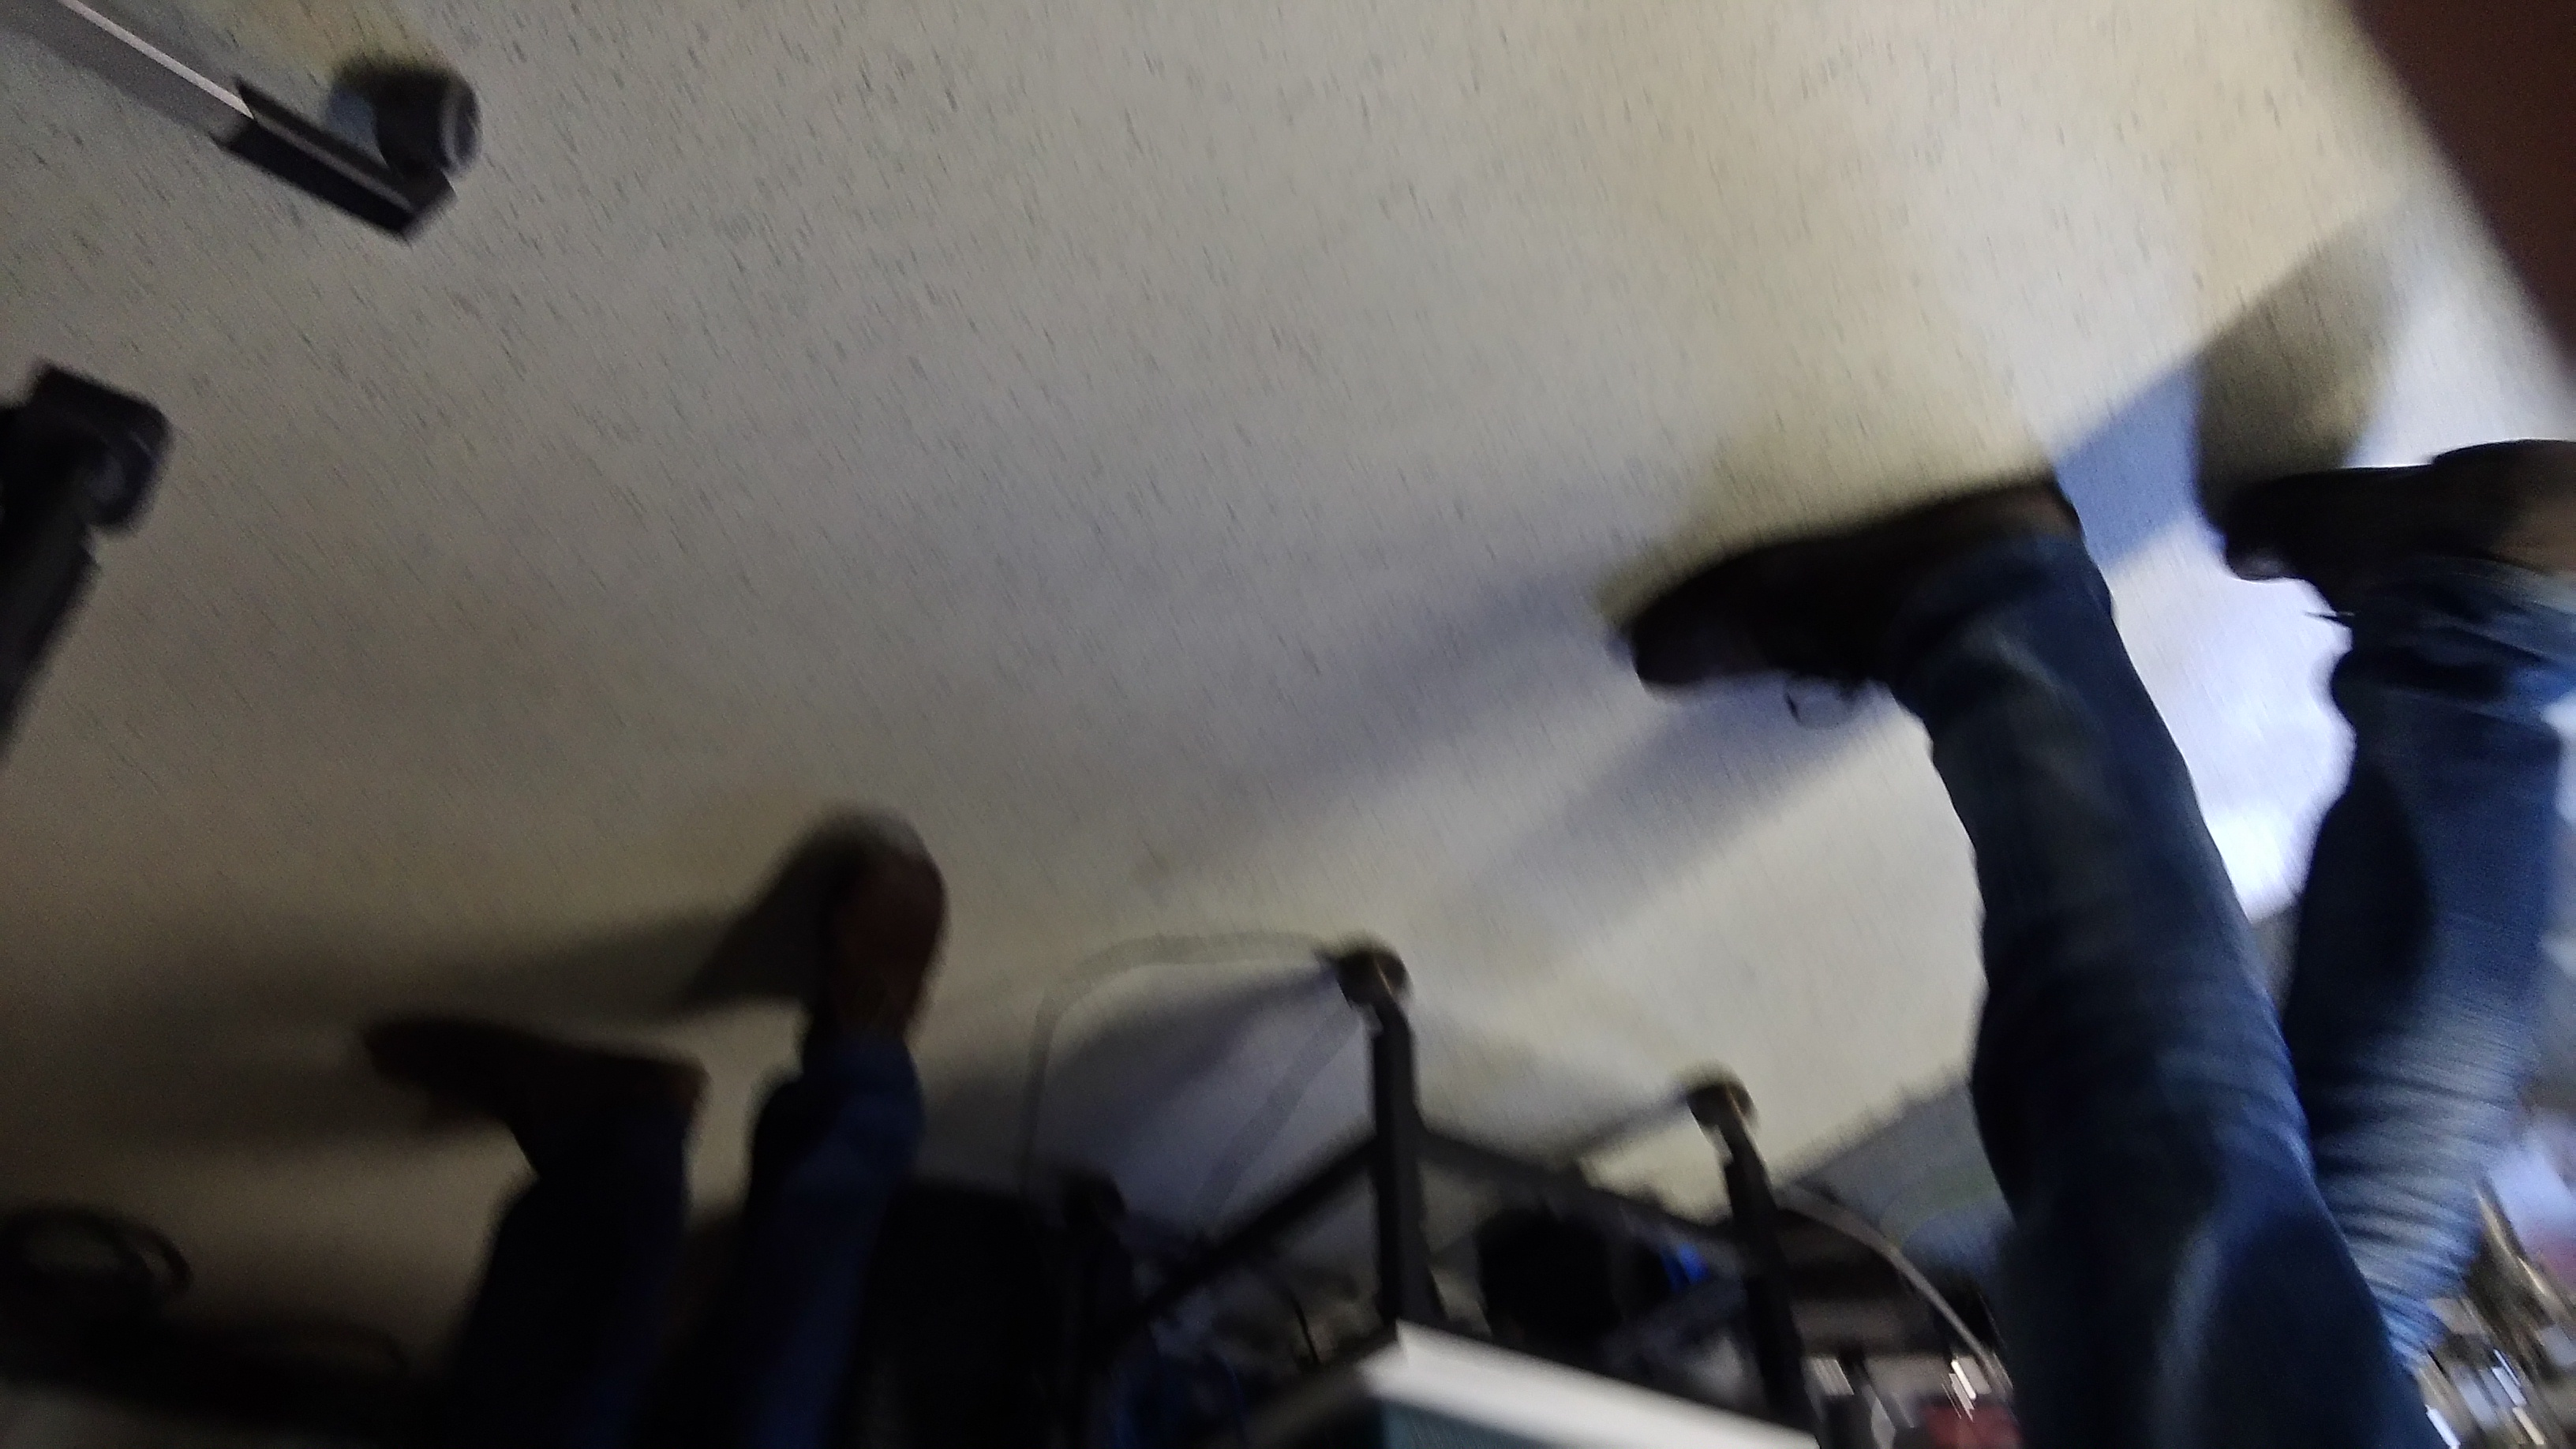
\includegraphics[width=\textwidth]{pictures/P_20150225_142813.jpg} \qquad
%  \caption{Der Versuchsaufbau}
% \end{center}
% \end{figure}

\begin{figure}[h]
\begin{center}
 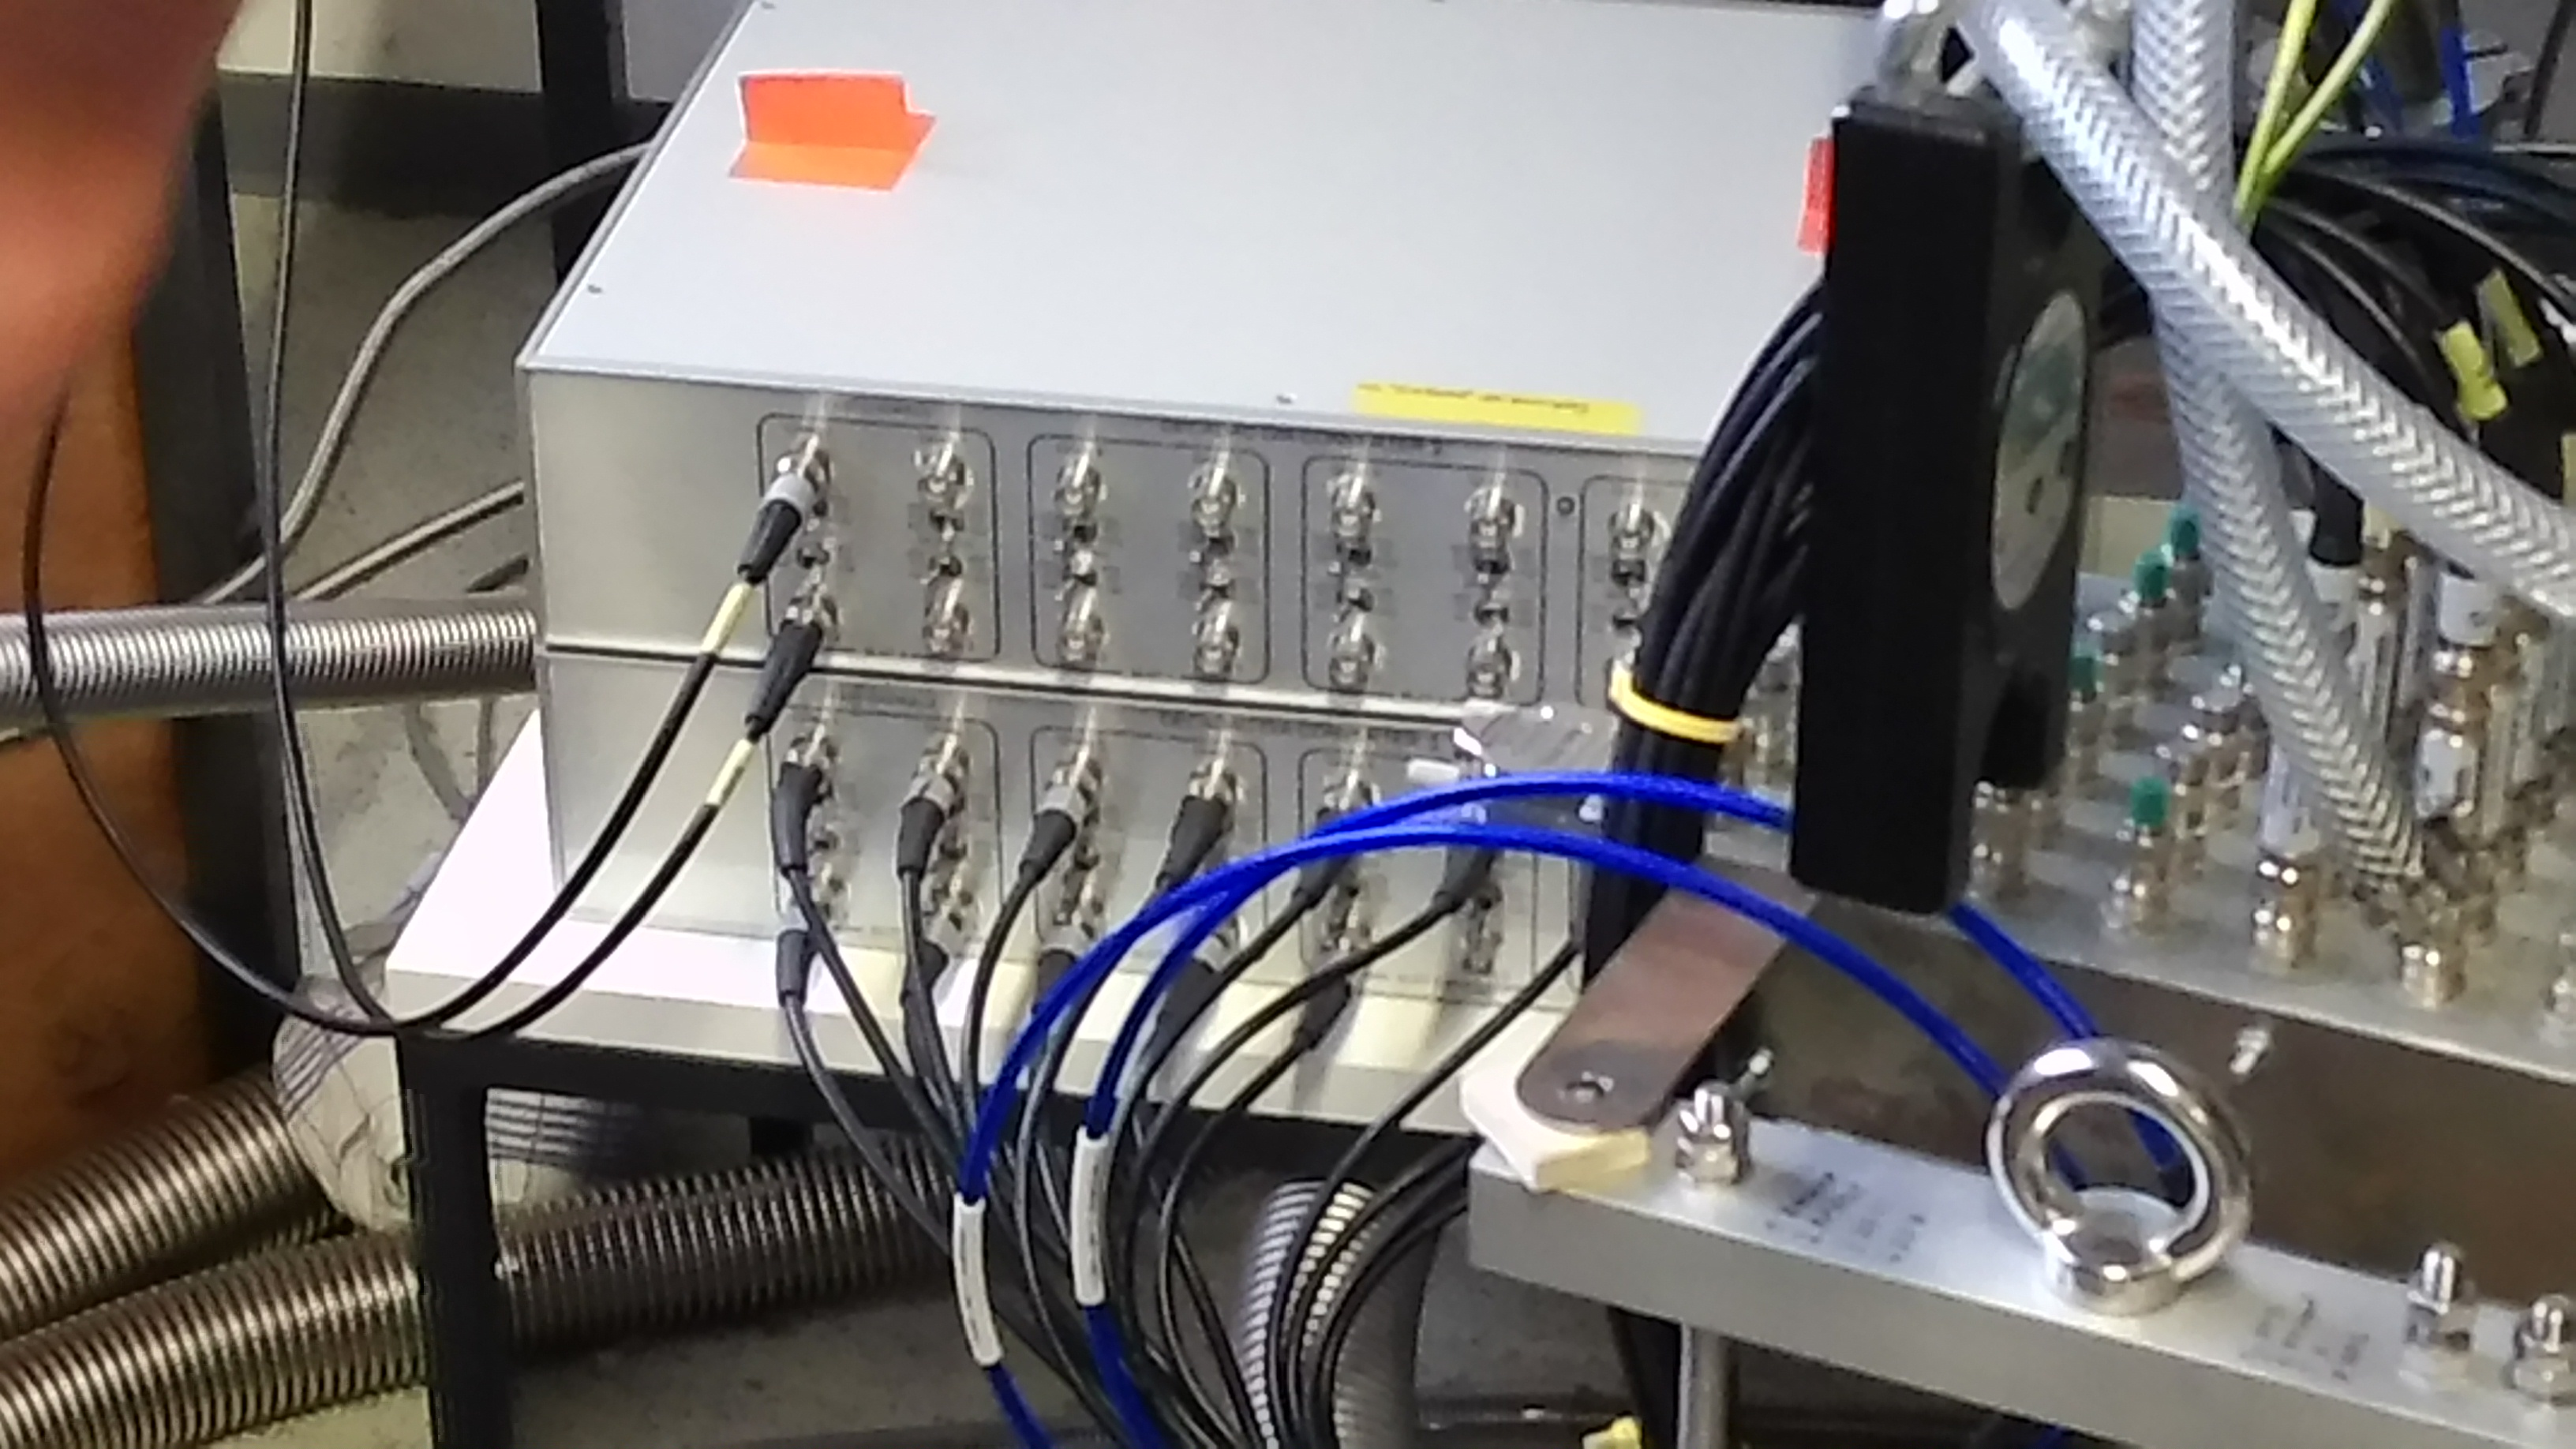
\includegraphics[width=\textwidth]{pictures/P_20150225_142923.jpg} \qquad
 \caption{Links: Gleichsspannungsversorgung, Rechts: Gefilterte Anschlüsse}
\end{center}
\end{figure}

\begin{figure}[h]
\begin{center}
 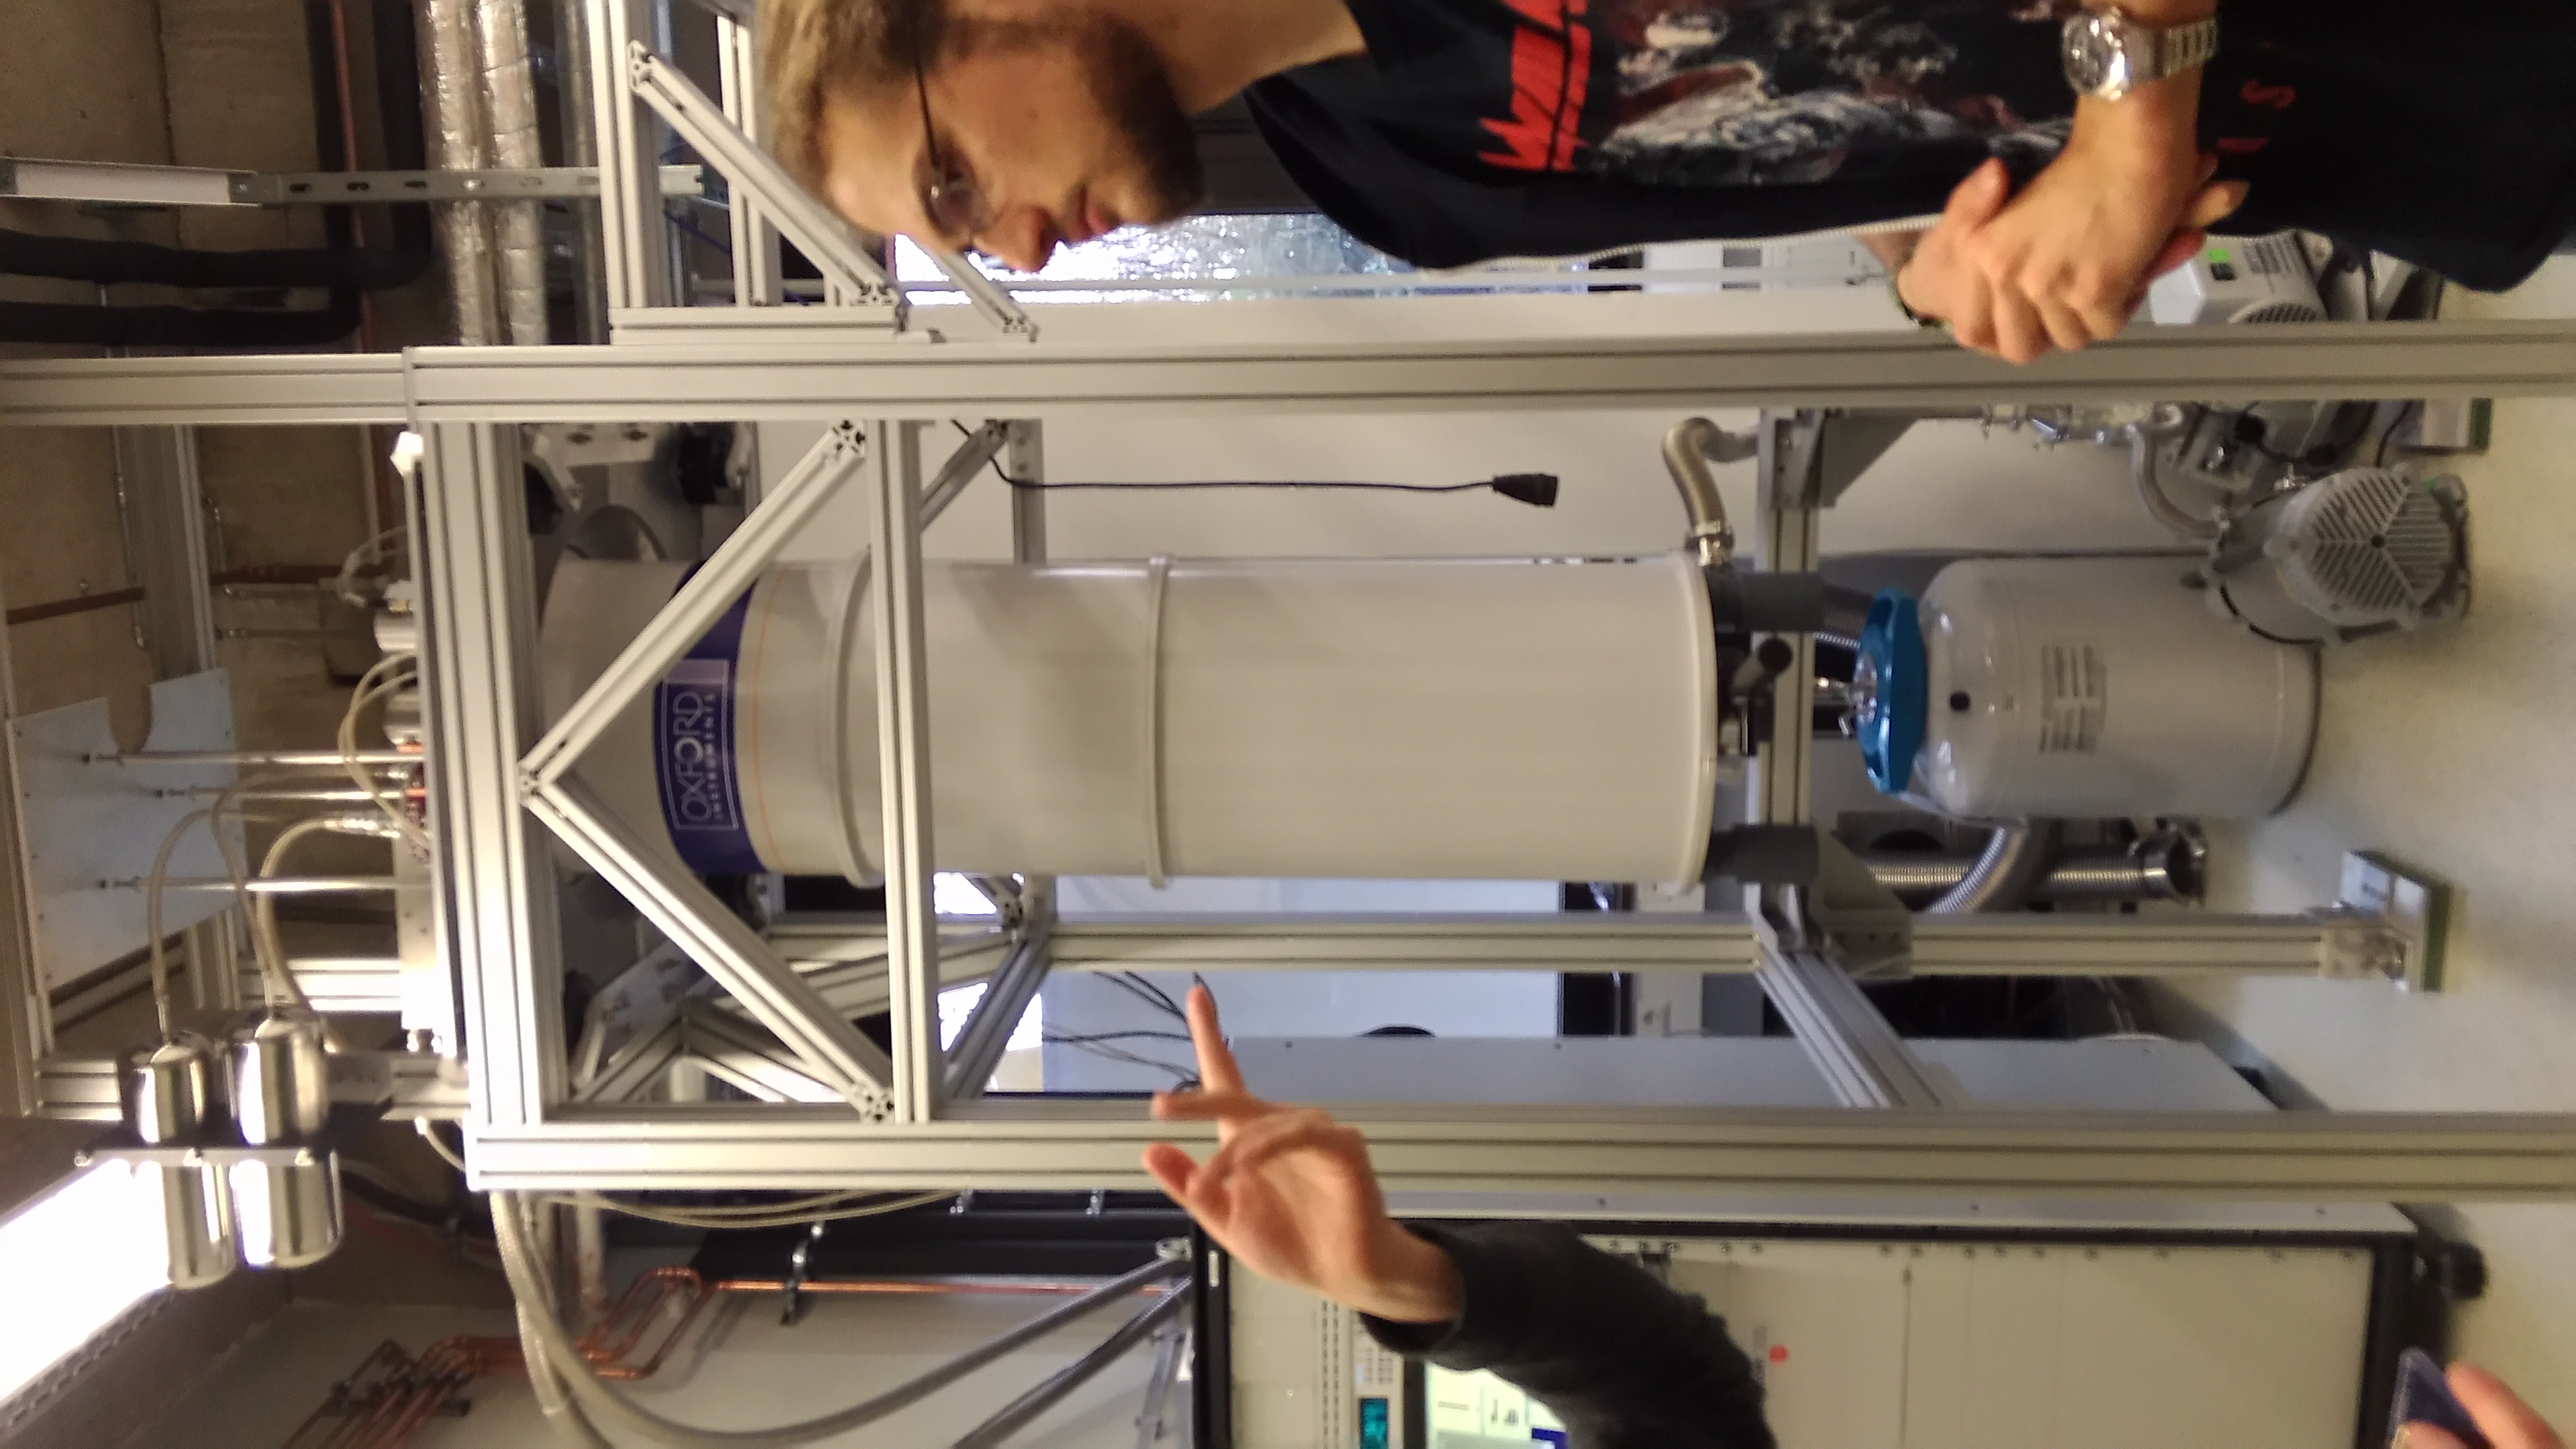
\includegraphics[width=\textheight,angle=270]{pictures/P_20150225_143154.jpg} \qquad
 \caption{Der untere Teil des Versuchsaufbaus. In dem weißen Behälter befindet sich dann der Chip.}
\end{center}
\end{figure}          

\begin{figure}[h]
\begin{center}
 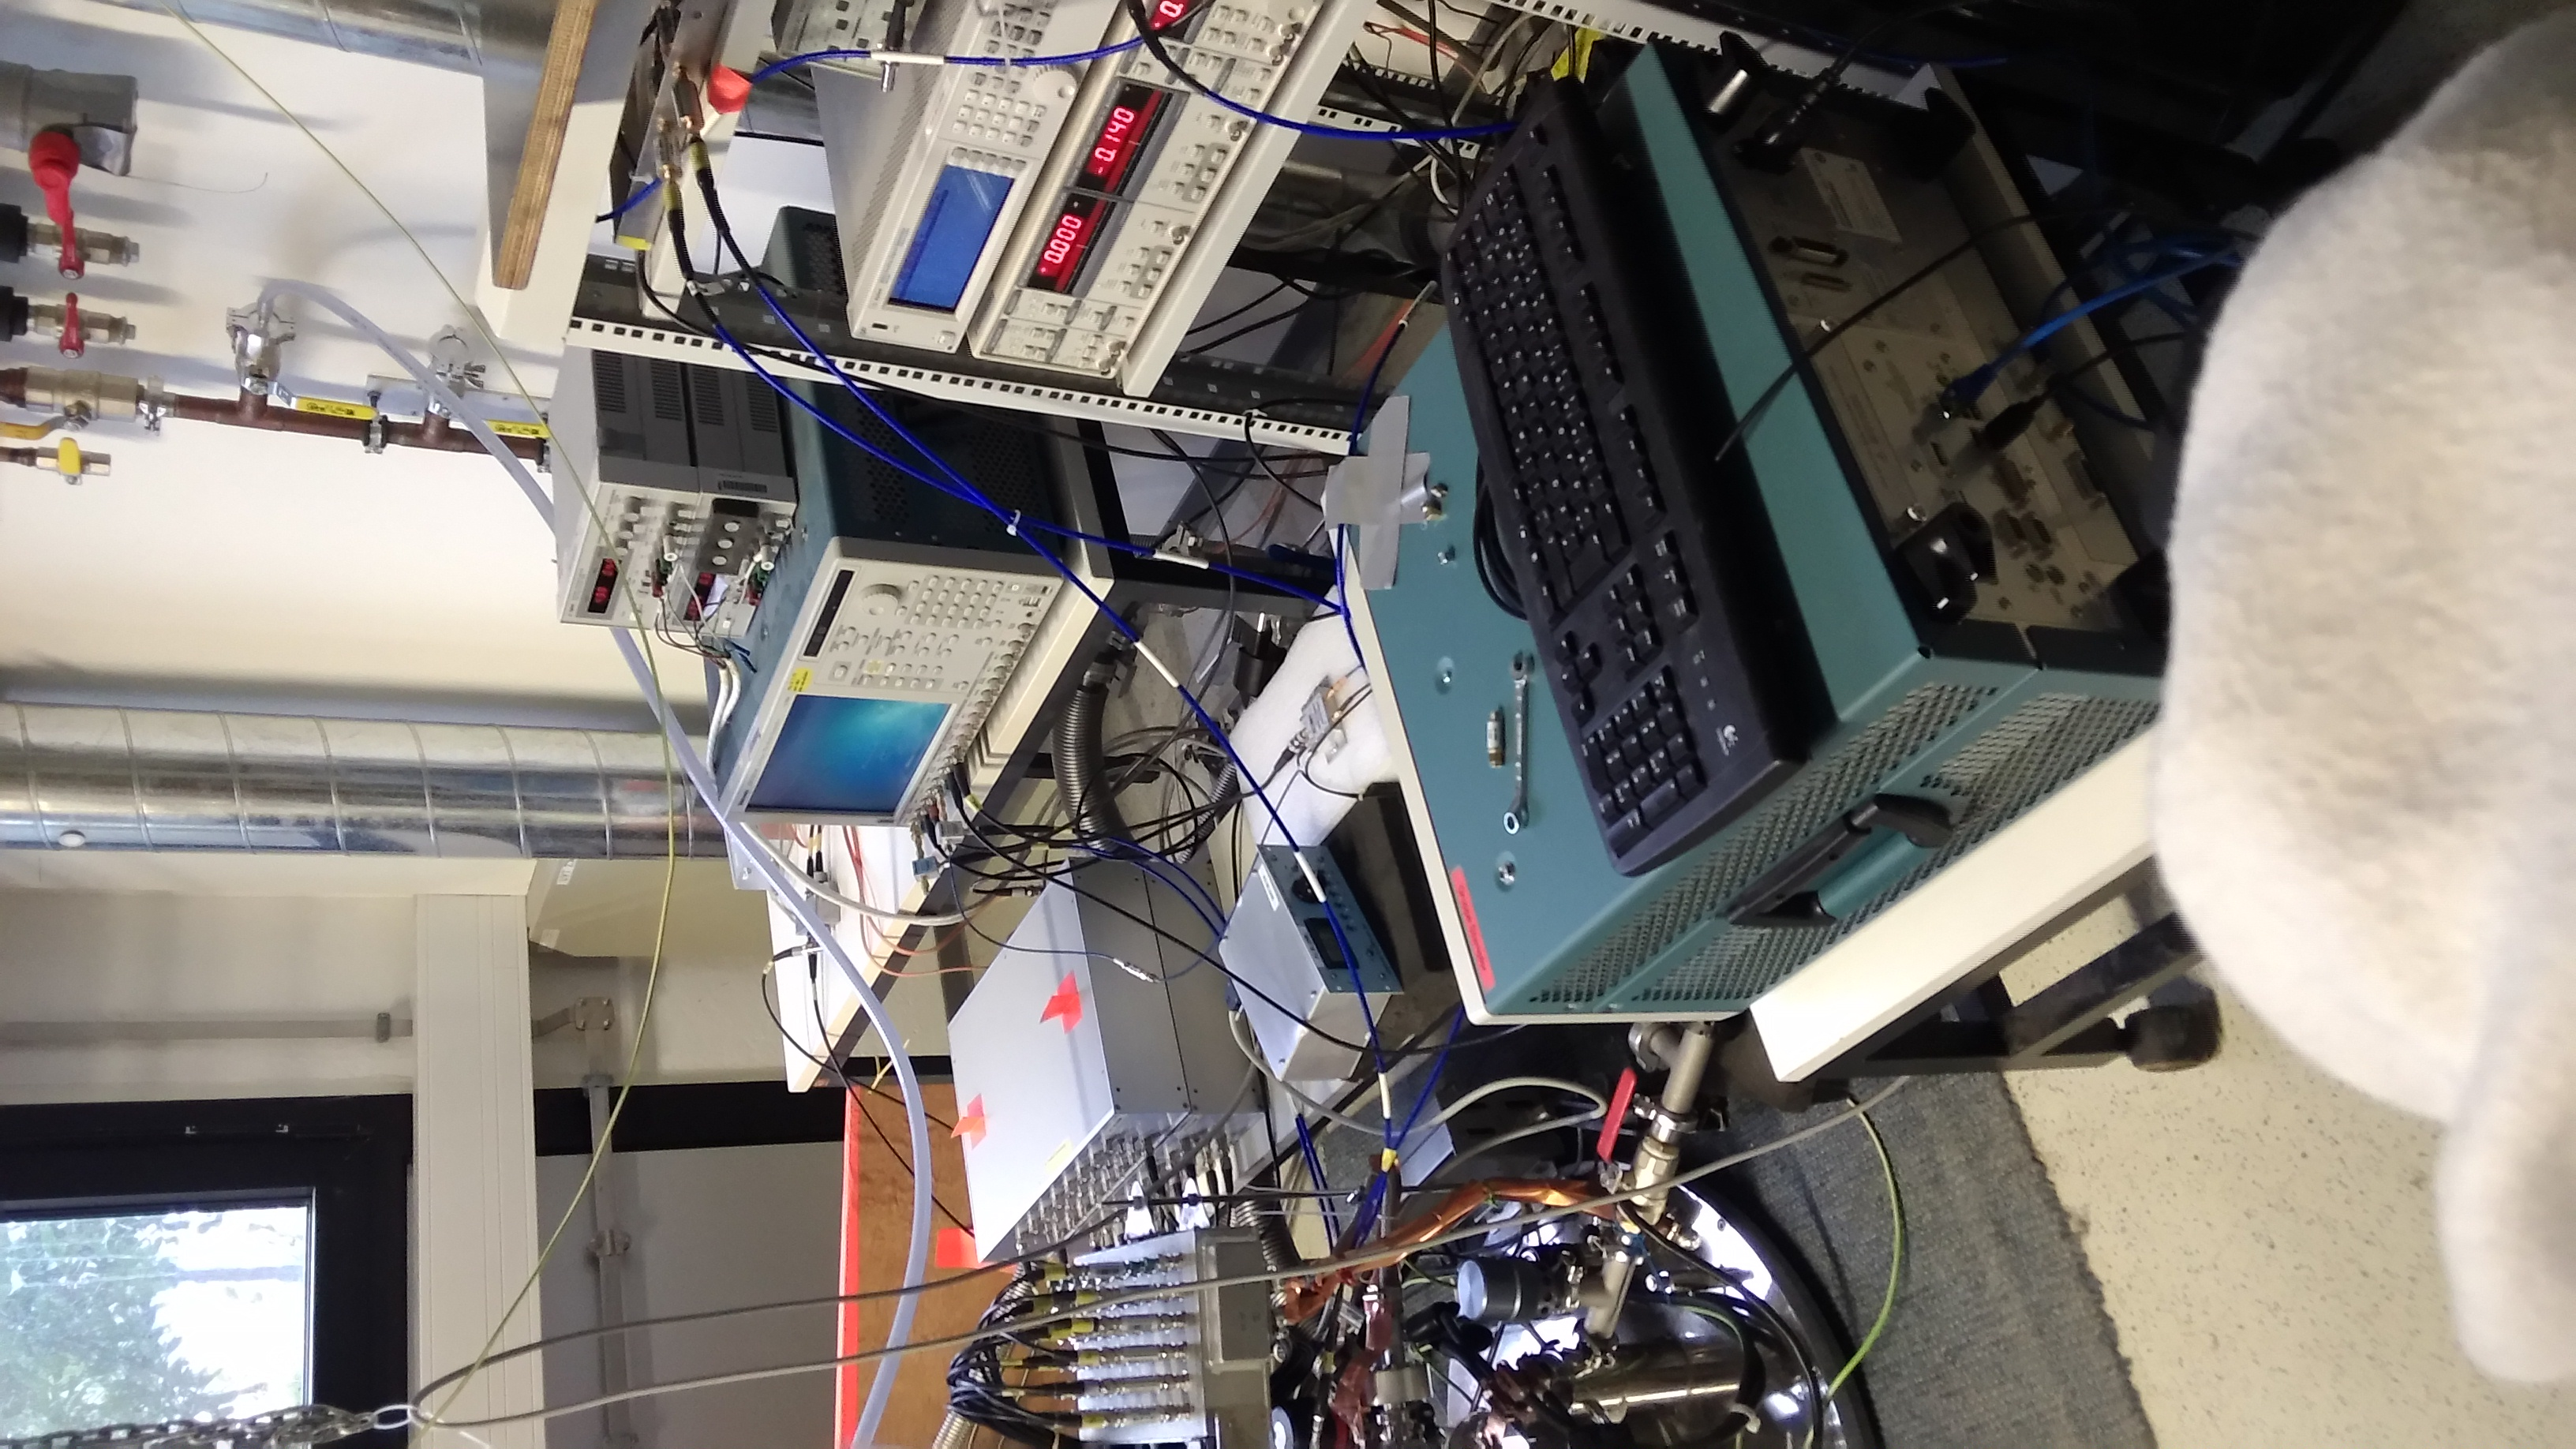
\includegraphics[width=\textheight,angle=270]{pictures/P_20150225_143557.jpg} \qquad
 \caption{Die beiden AWGs von Tectronix.}
\end{center}
\end{figure}


\begin{figure}[h]
\begin{center}
 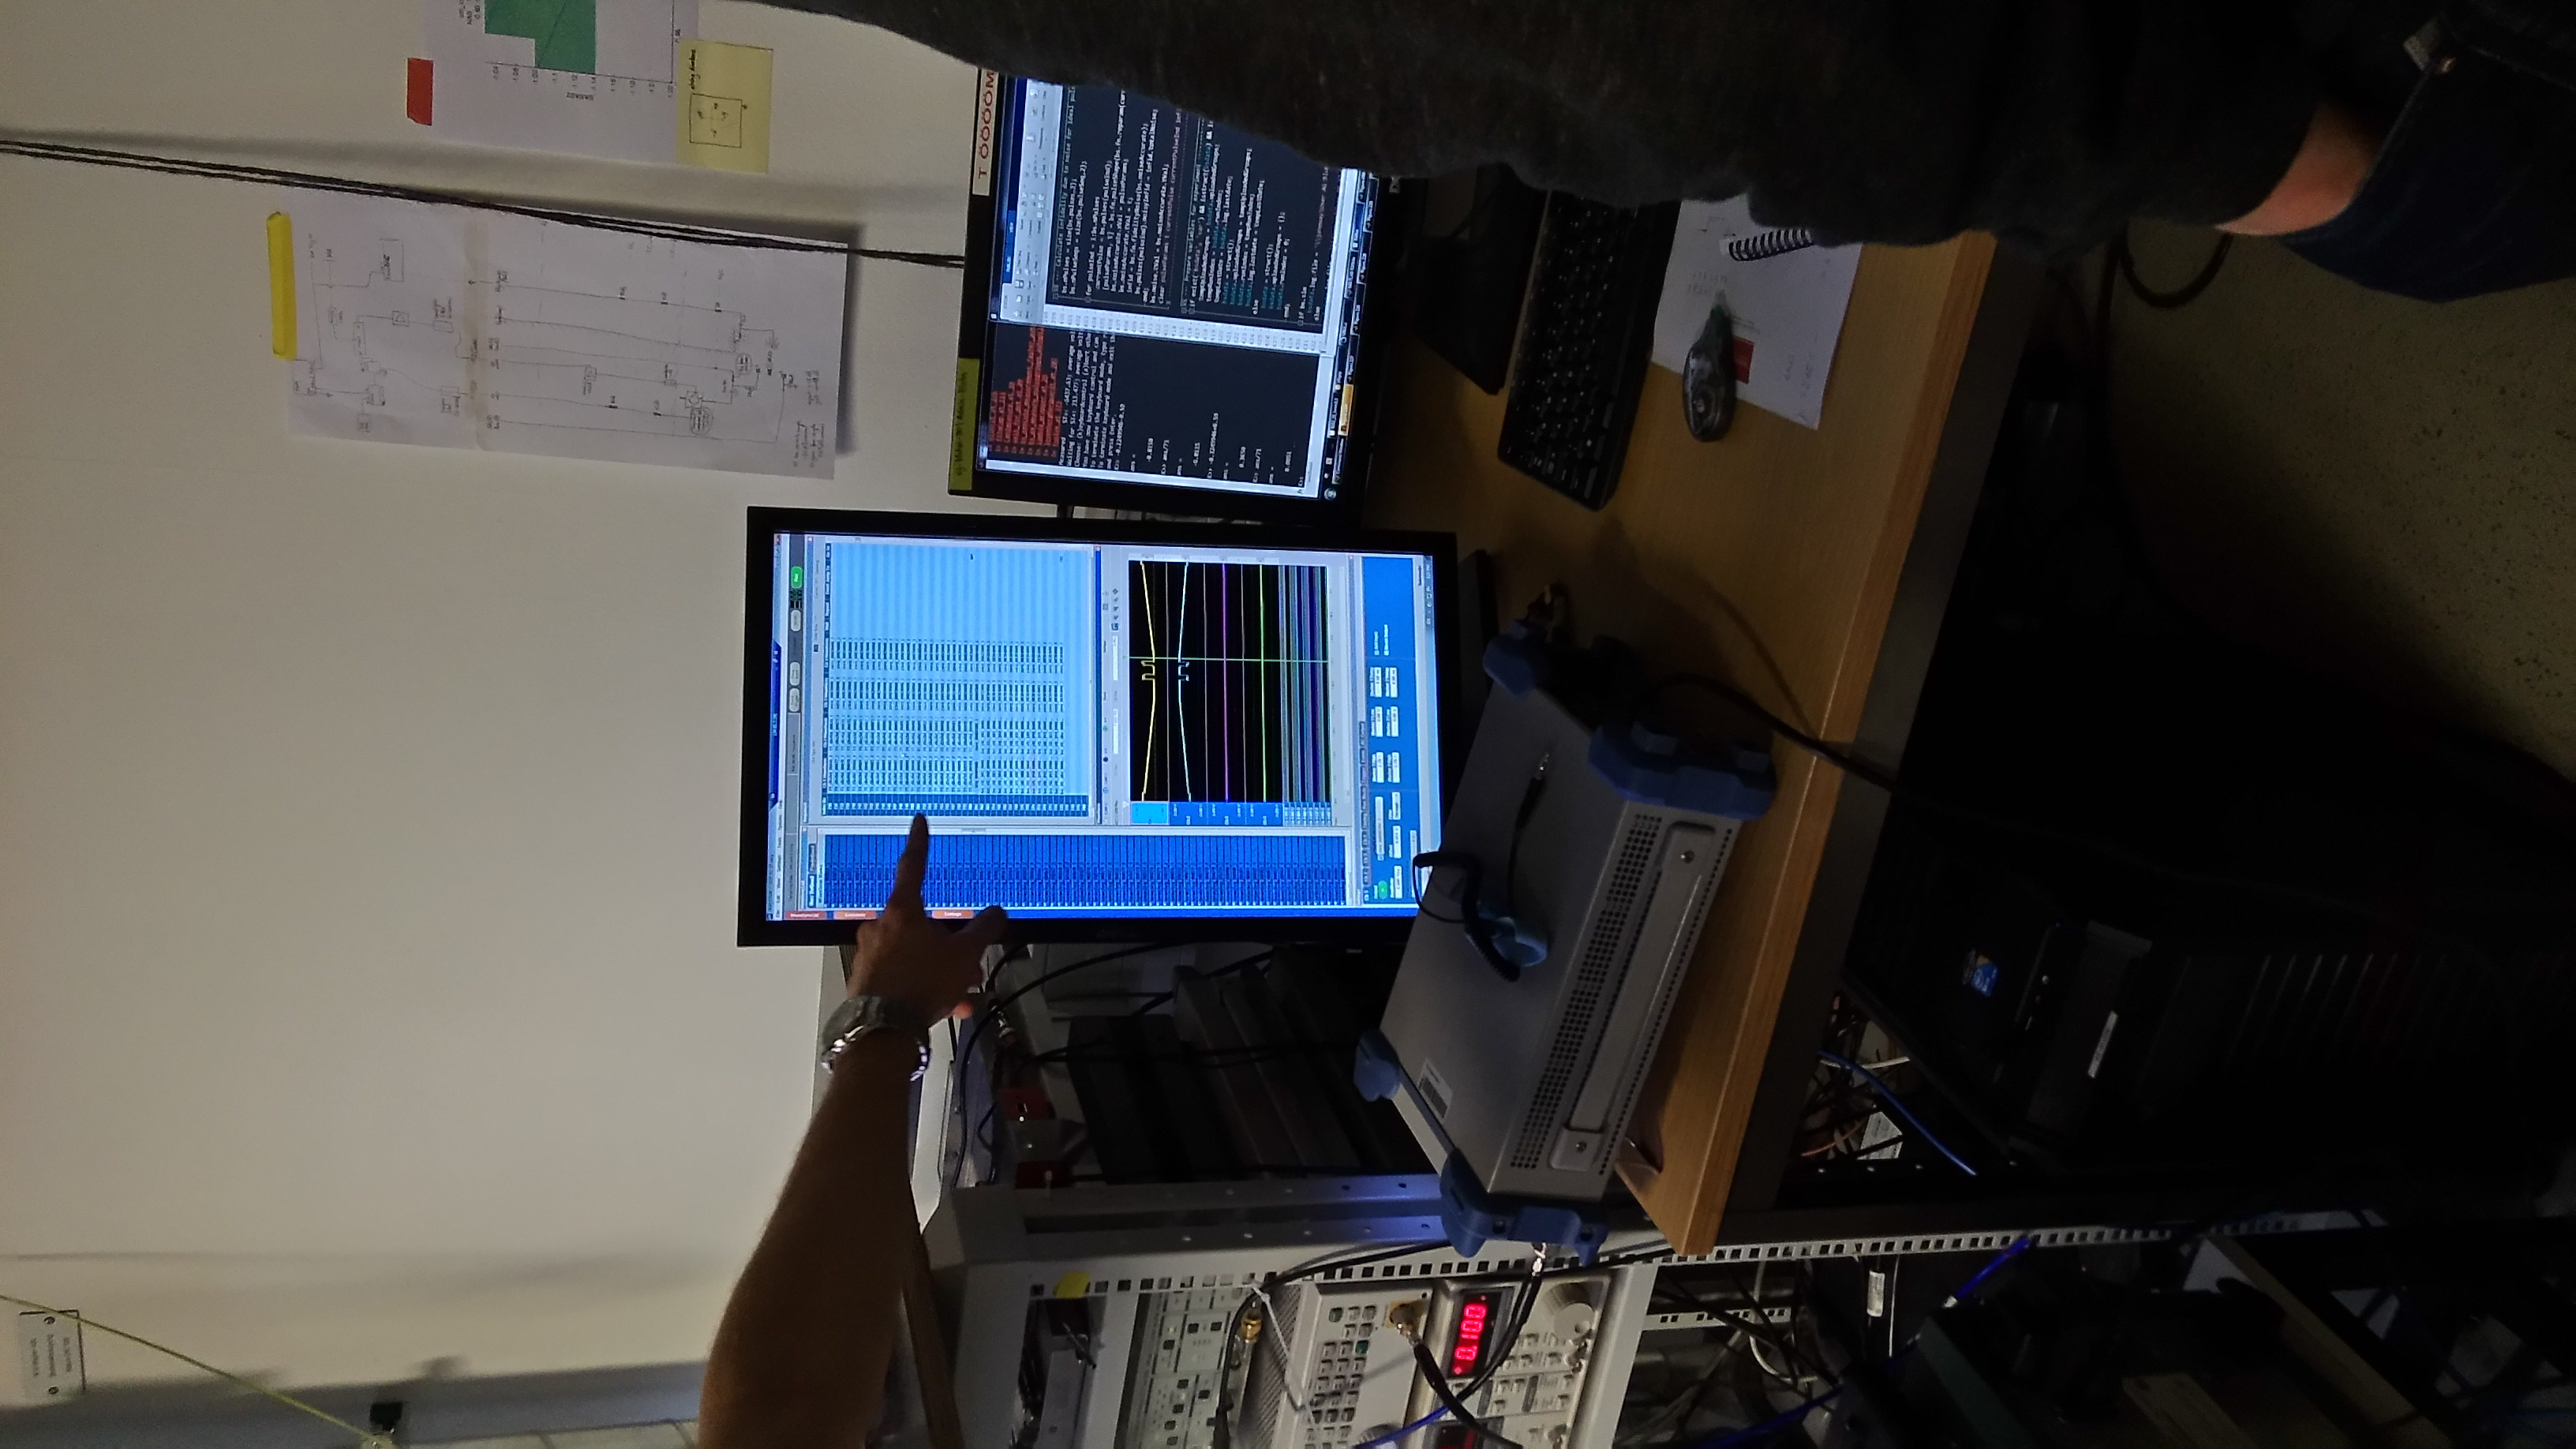
\includegraphics[width=\textheight, angle=270]{pictures/P_20150225_143613.jpg} \qquad
 \caption{Die GUI zur Auswahl der abszuspielenden Waveform mit unten Möglichkeit die Waveform zu betrachten. Per Remote (auf dem Gerät selber)}
\end{center}
\end{figure}          

\begin{figure}[h]
\begin{center}
 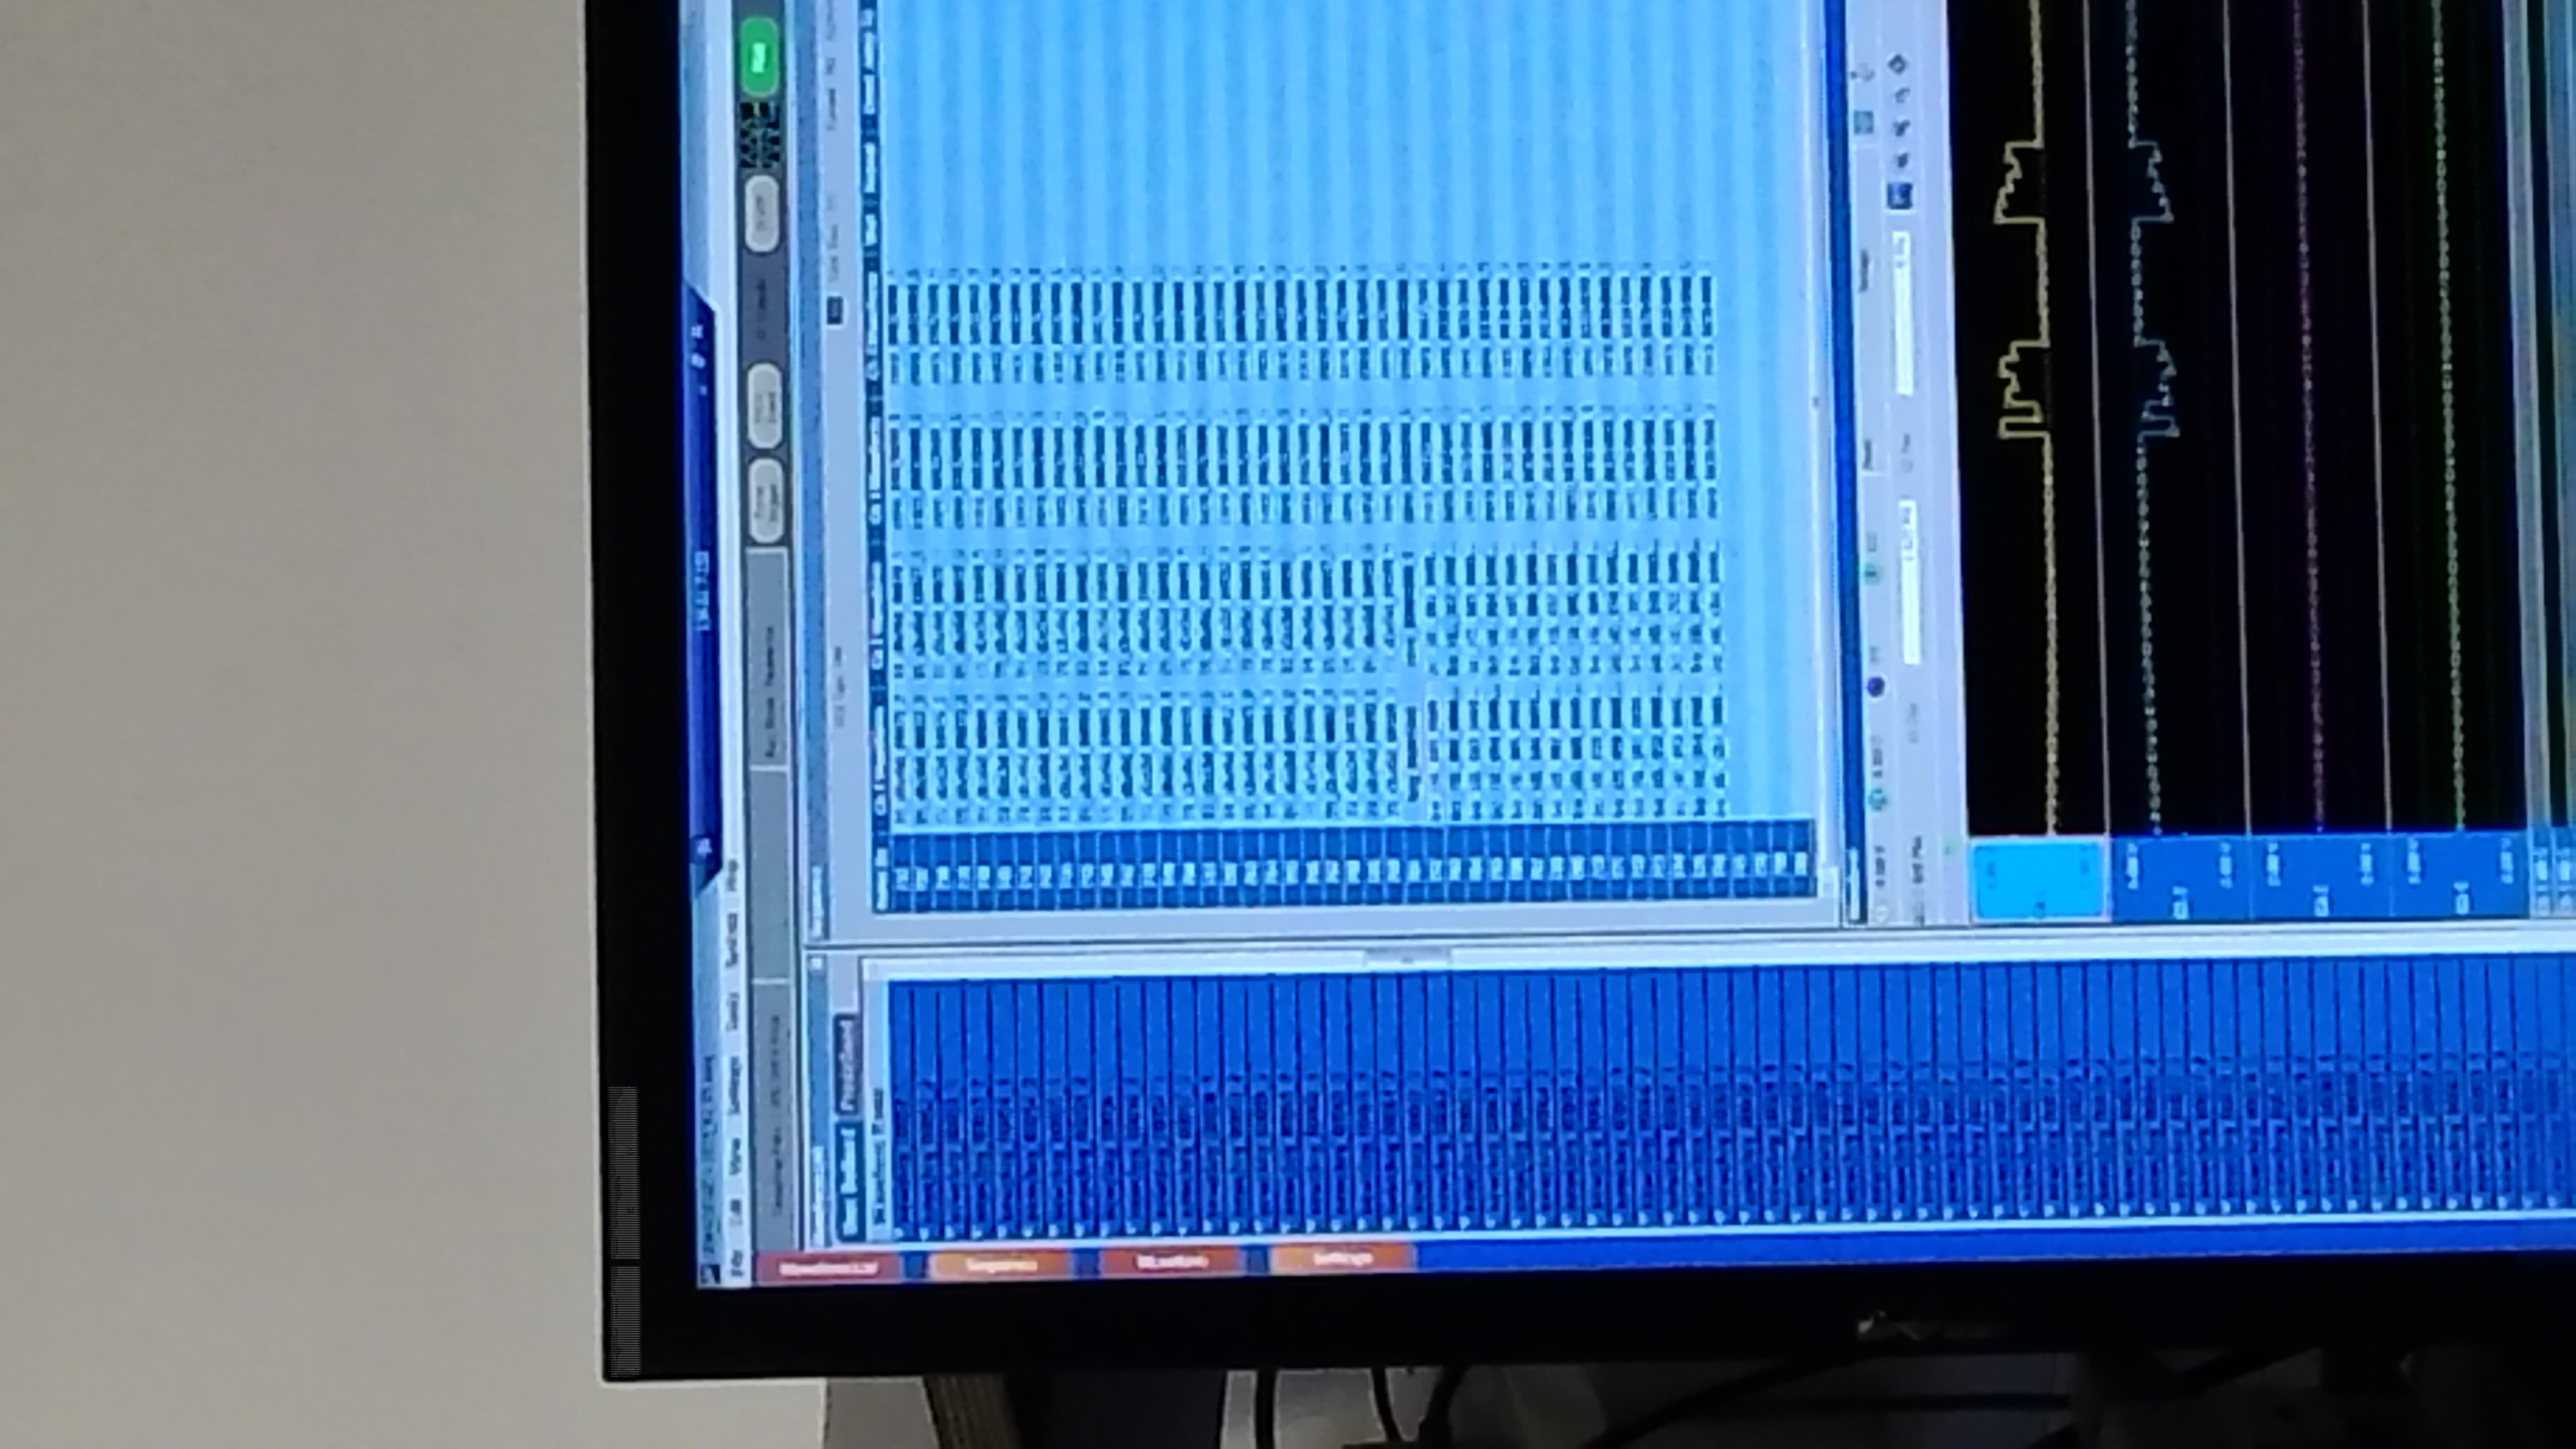
\includegraphics[width=\textheight,angle=270]{pictures/P_20150225_143734.jpg} \qquad
 \caption{Links: Alle zu verfügung stehenden Waveforms, Rechts: Indexierte (Dunkelblau) Waves (Hellblau) pro Spalte ein Kanal}
\end{center}
\end{figure}
\end{document}          
